\documentclass[12pt,a4paper,twoside]{article}



%language
%https://www.overleaf.com/learn/latex/German
\usepackage[utf8]{inputenc}                         %input encoding (umlaute)
\usepackage[T1]{fontenc}                            %correct encoding in resulting PDF
\usepackage[ngerman]{babel}                         %German-specific commands
\usepackage{csquotes}                               %quotation, https://www.overleaf.com/learn/latex/Typesetting_quotations

%document stuff
\usepackage[style=numeric]{biblatex}                %better than builtin bibtex, https://www.overleaf.com/learn/latex/Bibliography_management_with_biblatex
    \addbibresource{bibliography.bib}
\usepackage{fancyhdr}                               %custom header & footer, https://www.overleaf.com/learn/latex/Headers_and_footers
\usepackage{titling}                                %permanently available title, author, ...
\usepackage{lastpage}                               %total page number
\usepackage[margin=1in,headheight=28pt]{geometry}   %margins, headheight: 15/28pt for single/double line header
\usepackage{pdflscape}                              %single landscape pages, e.g. matplotlib outputs
\usepackage{pdfpages}                               %include PDFs, https://ctan.org/pkg/pdfpages?lang=en
\usepackage{hyperref}                               %links, https://www.overleaf.com/learn/latex/Hyperlinks

%math, physics
\usepackage{amsmath,amsthm,amsfonts,amssymb}        %equation formatting, theorems, fonts (blackboard), access to symbols, https://www.overleaf.com/learn/latex/Mathematical_expressions, https://www.overleaf.com/learn/latex/Theorems_and_proofs, https://www.overleaf.com/learn/latex/Mathematical_fonts, https://www.overleaf.com/learn/latex/List_of_Greek_letters_and_math_symbols
\usepackage[locale=DE,output-decimal-marker={,},separate-uncertainty=true,per-mode=symbol-or-fraction,range-phrase=-]{siunitx} %units, https://ctan.org/pkg/siunitx?lang=en
    %custom units
    \DeclareSIUnit\va{VA}                           %apparent power
    \DeclareSIUnit\var{var}                         %volt-ampere reactive
    \DeclareSIUnit\umdr{U}                          %revolutions
    \DeclareSIUnit\px{px}                           %pixel
    \DeclareSIUnit\torr{Torr}                       %torr

%tables
\usepackage{multirow}                               %multi row cells, for multicolumn no import is needed, https://www.overleaf.com/learn/latex/Tables#Combining_rows_and_columns
\usepackage{array}                                  %fixed sized cells, https://www.overleaf.com/learn/latex/Tables#Tables_with_fixed_length
\usepackage{float}                                  %positioning, https://www.overleaf.com/learn/latex/Positioning_of_Figures
\usepackage{longtable}                              %multipage tables, https://www.overleaf.com/learn/latex/Tables#Multi-page_tables

%graphics
\usepackage{graphicx}                               %graphics, https://www.overleaf.com/learn/latex/Inserting_Images
    \graphicspath{ {./images/} }                        %images in subfolder to keep root clean
\usepackage{caption}                                %more caption options
\usepackage{subcaption}                             %captions of subfigures
    \captionsetup[table]{skip=6pt}
%\usepackage{tikz}                                   %generate graphics, https://www.overleaf.com/learn/latex/TikZ_package
%\usepackage{pgfplots}                               %generate plots, https://www.overleaf.com/learn/latex/Pgfplots_package
%    \pgfplotsset{compat=1.9}
%\usepackage{epic}                                   %better picture mode, https://ctan.org/pkg/epic?lang=en

%disciplines other than math & physics
\usepackage[version=4]{mhchem}                      %simpler to use than chemfig, https://www.overleaf.com/learn/latex/Chemistry_formulae

%utility
\usepackage{todonotes}                              %todo annotations
\usepackage[normalem]{ulem}                         %strike through text



%custom operators, https://www.overleaf.com/learn/latex/Operators#Defining_your_own_operators
\DeclareMathOperator{\arsinh}{arsinh}               %trig
\DeclareMathOperator{\arcosh}{arcosh}
\DeclareMathOperator{\artanh}{artanh}
\DeclareMathOperator{\grad}{grad}                   %multivariate analysis
\let\div\relax
\DeclareMathOperator{\div}{div}
\DeclareMathOperator{\rot}{rot}
\DeclareMathOperator{\dom}{dom}                     %functional analysis
\DeclareMathOperator{\ran}{ran}
\DeclareMathOperator{\Vol}{Vol}
\DeclareMathOperator{\Res}{Res}
\DeclareMathOperator{\Avg}{Avg}                     %staticstics
\DeclareMathOperator{\Var}{Var}
\DeclareMathOperator{\StD}{StD}
\DeclareMathOperator{\CoV}{CoV}
\DeclareMathOperator{\sgn}{sgn}                     %other
\DeclareMathOperator{\tr}{tr}

%theorems, https://www.overleaf.com/learn/latex/Theorems_and_proofs
\theoremstyle{definition}
\newtheorem{definition}{Definition}[section]
\newtheorem{bemerkung}{Bemerkung}[definition]
\newtheorem{satz}{Satz}[section]
\newtheorem{lemma}{Lemma}[section]
\newtheorem{proposition}{Proposition}[section]
\newtheorem{korollar}{Korollar}[section]

%math columns, https://tex.stackexchange.com/q/257128
\newcolumntype{L}{>{$}l<{$}}
\newcolumntype{C}{>{$}c<{$}}
\newcolumntype{R}{>{$}r<{$}}



\title{Labor 2 \\ TU6: Transformator}
\author{Gruppe 4: \\ Angermann \& Gössl}
\date{20WS \\ 04.02.2021}
%adjust headheight: 15/28pt for single/double line header


\pagestyle{fancyplain}
\fancyhead[L]{\thedate}
\fancyhead[C]{\theauthor}
\fancyhead[R]{\thetitle}
\fancyfoot[C]{\thepage{ }/ \pageref*{LastPage}}




\begin{document}



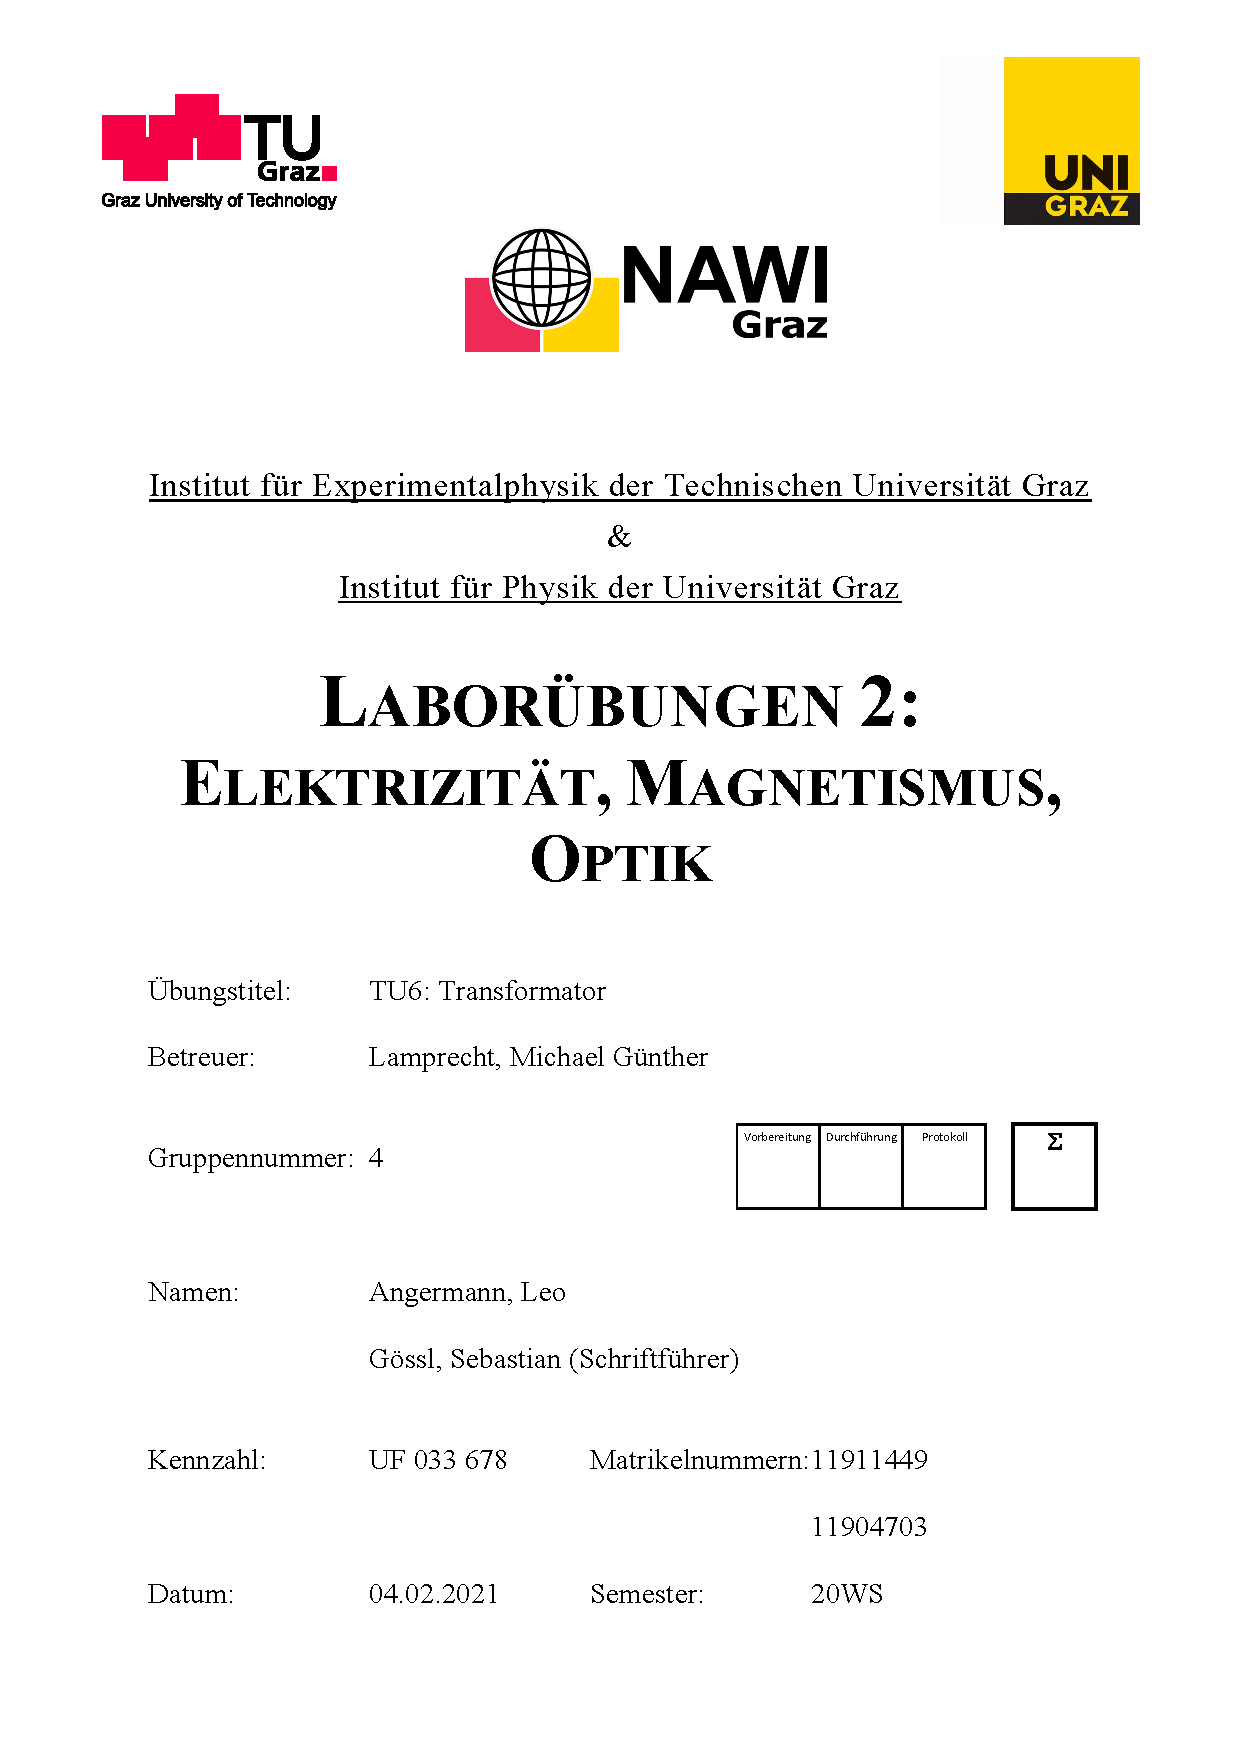
\includepdf{Deckblatt}



\tableofcontents
\newpage



\section*{Anmerkung}

Das Titelblatt (vom Autor ausgefüllt) und die ersten beiden Kapitel (und das dritte teilweise) wurden bereitgestellt \cite{teachcenter2}.



\section{Aufgabenstellung}

Die Messungen werden mit der in Abb. 9 dargestellten Schaltung durchgeführt. Überlastungen des elektronischen Leistungsmessers sind zu vermeiden (siehe Bedienungsanleitung), richtigen Meßbereich für Strom und Spannung sind jeweils einzustellen.

\begin{enumerate}
    \item Leerlauf ($U=\SI{160}{\V}$): Messen Sie Primärstrom $I_1$, Primärspannung $U_1$, Wirkleistung $P_1$ und Sekundäspannung $U_2$. Berechnen Sie die Größen aus Tab. 1, Fehlerrechnung. Oszillographische Darstellung von Primärstrom und Sekundärspannung mit passender Skalierung.
    \item Ohm’sche Last sekundärseitig (ca. $I_2 < \SI{1}{\ampere}$): Messen Sie Primärstrom, Primärspannung, Wirkleistung, Sekundärspannung und Sekundärstrom $I_2$. Berechnen Sie die Größen aus Tab. 1, Fehlerrechnung. Oszillographische Darstellung von Primärstrom und Sekundärspannung mit passender Skalierung.
    \item Ohm’sch-induktive Last: Aufnahme der Parameter wie unter Aufgabe 2 bei einer Serienschaltung von einer Spule $L\approx\SI{0,1}{\henry}$ mit einem regelbaren Lastwiderstand (\SIrange{0}{45}{\ohm}, ca. 20 Meßwerte). Erstellung des Diagrammes Leistung über Lastwiderstand und Begründung des Auftretens eines Maximums der Wirkleistung. Oszillographisches Bild beim Maximum abzeichnen und skalieren!
    \item \sout{Ohm’sch-kapazitive Last [\dots]}
    \item Die Fehlerrechnung ist für einen der Punkte 3 \sout{oder 4} durchzuführen.
\end{enumerate}
\begin{table}[H]
    \centering
    \caption{Zu berechnende Größen für Aufgabe 1 und 2.}
    \label{tab:aufgabe}
    \begin{tabular}{r C | r C}
        Scheinleistung primär               & S_1 = U_1 I_1                                 & Blindleistung primär  & Q_1 = \sqrt{S_1^2 - P_1^2} \\
        \multirow{2}{*}{Leistungsfaktor}    & \multirow{2}{*}{$\cos\phi = \frac{P_1}{S_1}$} & Wirkleistung sekundär & \multirow{2}{*}{$P_2 = U_2 I_2$} \\
                                            &                                               & (bei ohm’scher Last)  & \\
        Verlustleistung gesamt              & P_V = P_1 - P_2                               & Wirkungsgrad          & \eta = \frac{P_2}{P_1}
    \end{tabular}
\end{table}



\section{Voraussetzungen \& Grundlagen}

Ist eine Wechselspannung $U_1$ vorhanden, deren Höhe für einen bestimmten Zweck ungeeignet
ist, so wird ein Umspanner Abb. 1 verwendet.
\begin{figure}[H]
    \centering
    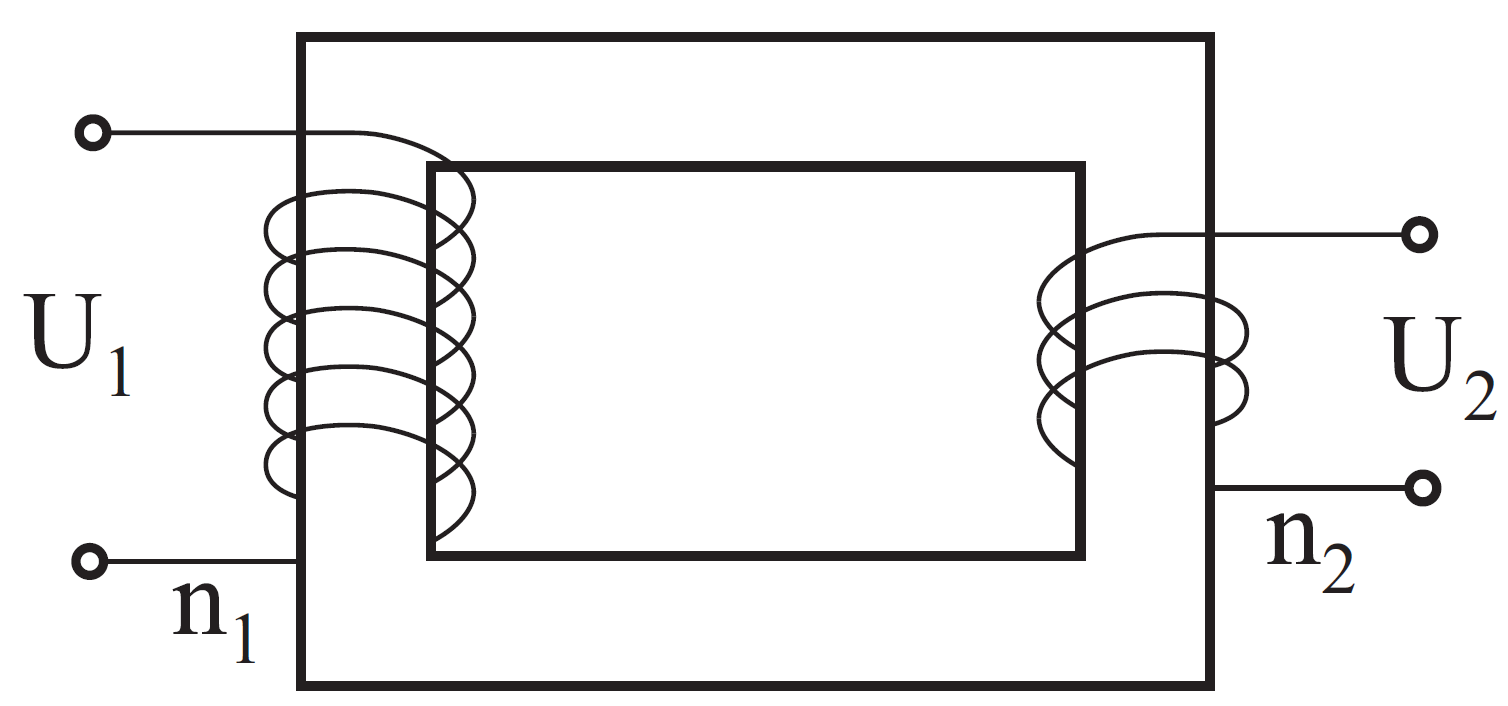
\includegraphics[width=\linewidth/3]{grundlagen/abb1}
    \caption{Umspanner, Transformator. [Eisenkern eines klassischen Transformators. Links mit der Primärspule, bestehend aus $n_1$ Windungen und gespeißt mit Spannung $U_1$, und rechts mit der Sekundärspule, aus $n_2$ Windungen und einer induzierten Spannung $U_2$.]}
\end{figure}
Die Netzspannung
\begin{equation}
    U_1 = U_0 \sin \omega t
\end{equation}
erzeugt einen Strom $I_1(t)$ im Primärkreis. Dieser Strom bewirkt einen magnetischen Fluß $\Phi(t)$ in der Spule. Die Flußänderung induziert eine Spannung $U_L$ in der Spule.
\begin{equation}
    U_L = - n_1 \frac{d \Phi}{d t}
\end{equation}
Für den Primärkreis gilt also:
\begin{gather}
    U_1 + U_L = 0 \\
    U_0 \sin \omega t = n_1 \frac{d \Phi}{d t}
\end{gather}
Damit ist der magnetische Fluß $\Phi(t)$ durch die Netzspannung $U_1(t)$ vorgegeben.


\subsection{Leerlauf}

$I_2 = 0$. Die Flußänderung induziert in der Sekundärspule eine Spannung $U_2$:
\begin{gather}
    U_2 = -n_2 \frac{d \Phi}{d t} = - \frac{n_2}{n_1} U_0 \sin \omega t \\
    U_2 = - \frac{n_2}{n_1} U_1(t)
\end{gather}
Das Verhältnis der Spannungen ist somit durch die Windungszahlen gegeben. Der Strom im Primärkreis wird nur durch das Magnetisierungsverhalten des Eisens festgelegt.
\begin{equation}
    \Phi = B A = \mu \mu_0 H A = \mu \mu_0 \frac{A}{l} n_1 I_1
\end{equation}
Bei geradliniger Magnetisierungskurve des verwendeten Eisens (Abb. 2) ist der Strom dem von ihm hervorgerufenen Fluß proportional. Es wird daher auch die Stromwelle der angelegten Spannung um $\pi/2$ nacheilen. Die elektrische Leistung eines Gerätes ist durch das Produkt von Spannung und Strom gegeben. Die Leistung $N$ an der Primärspule in Abhängigkeit von der Zeit bei Nacheilung des Stromes gegenüber der Spannung um $\pi/2$ zeigt Abb. 3. Man erkennt, daß das Vorzeichen der Leistung wechselt. Die aufgenommene Arbeit wird also stets wieder an das Netz zurückgegeben. Man nennt das Produkt $U_1 I_b$ im Falle einer Phasenverschiebung von $\pi/2$ Blindleistung $Q_1$. Der aufgenommene Blindstrom $I_b$ wird Magnetisierungsstrom genannt.
\begin{figure}[H]
    \centering
    \begin{minipage}[b]{0.45\textwidth}
        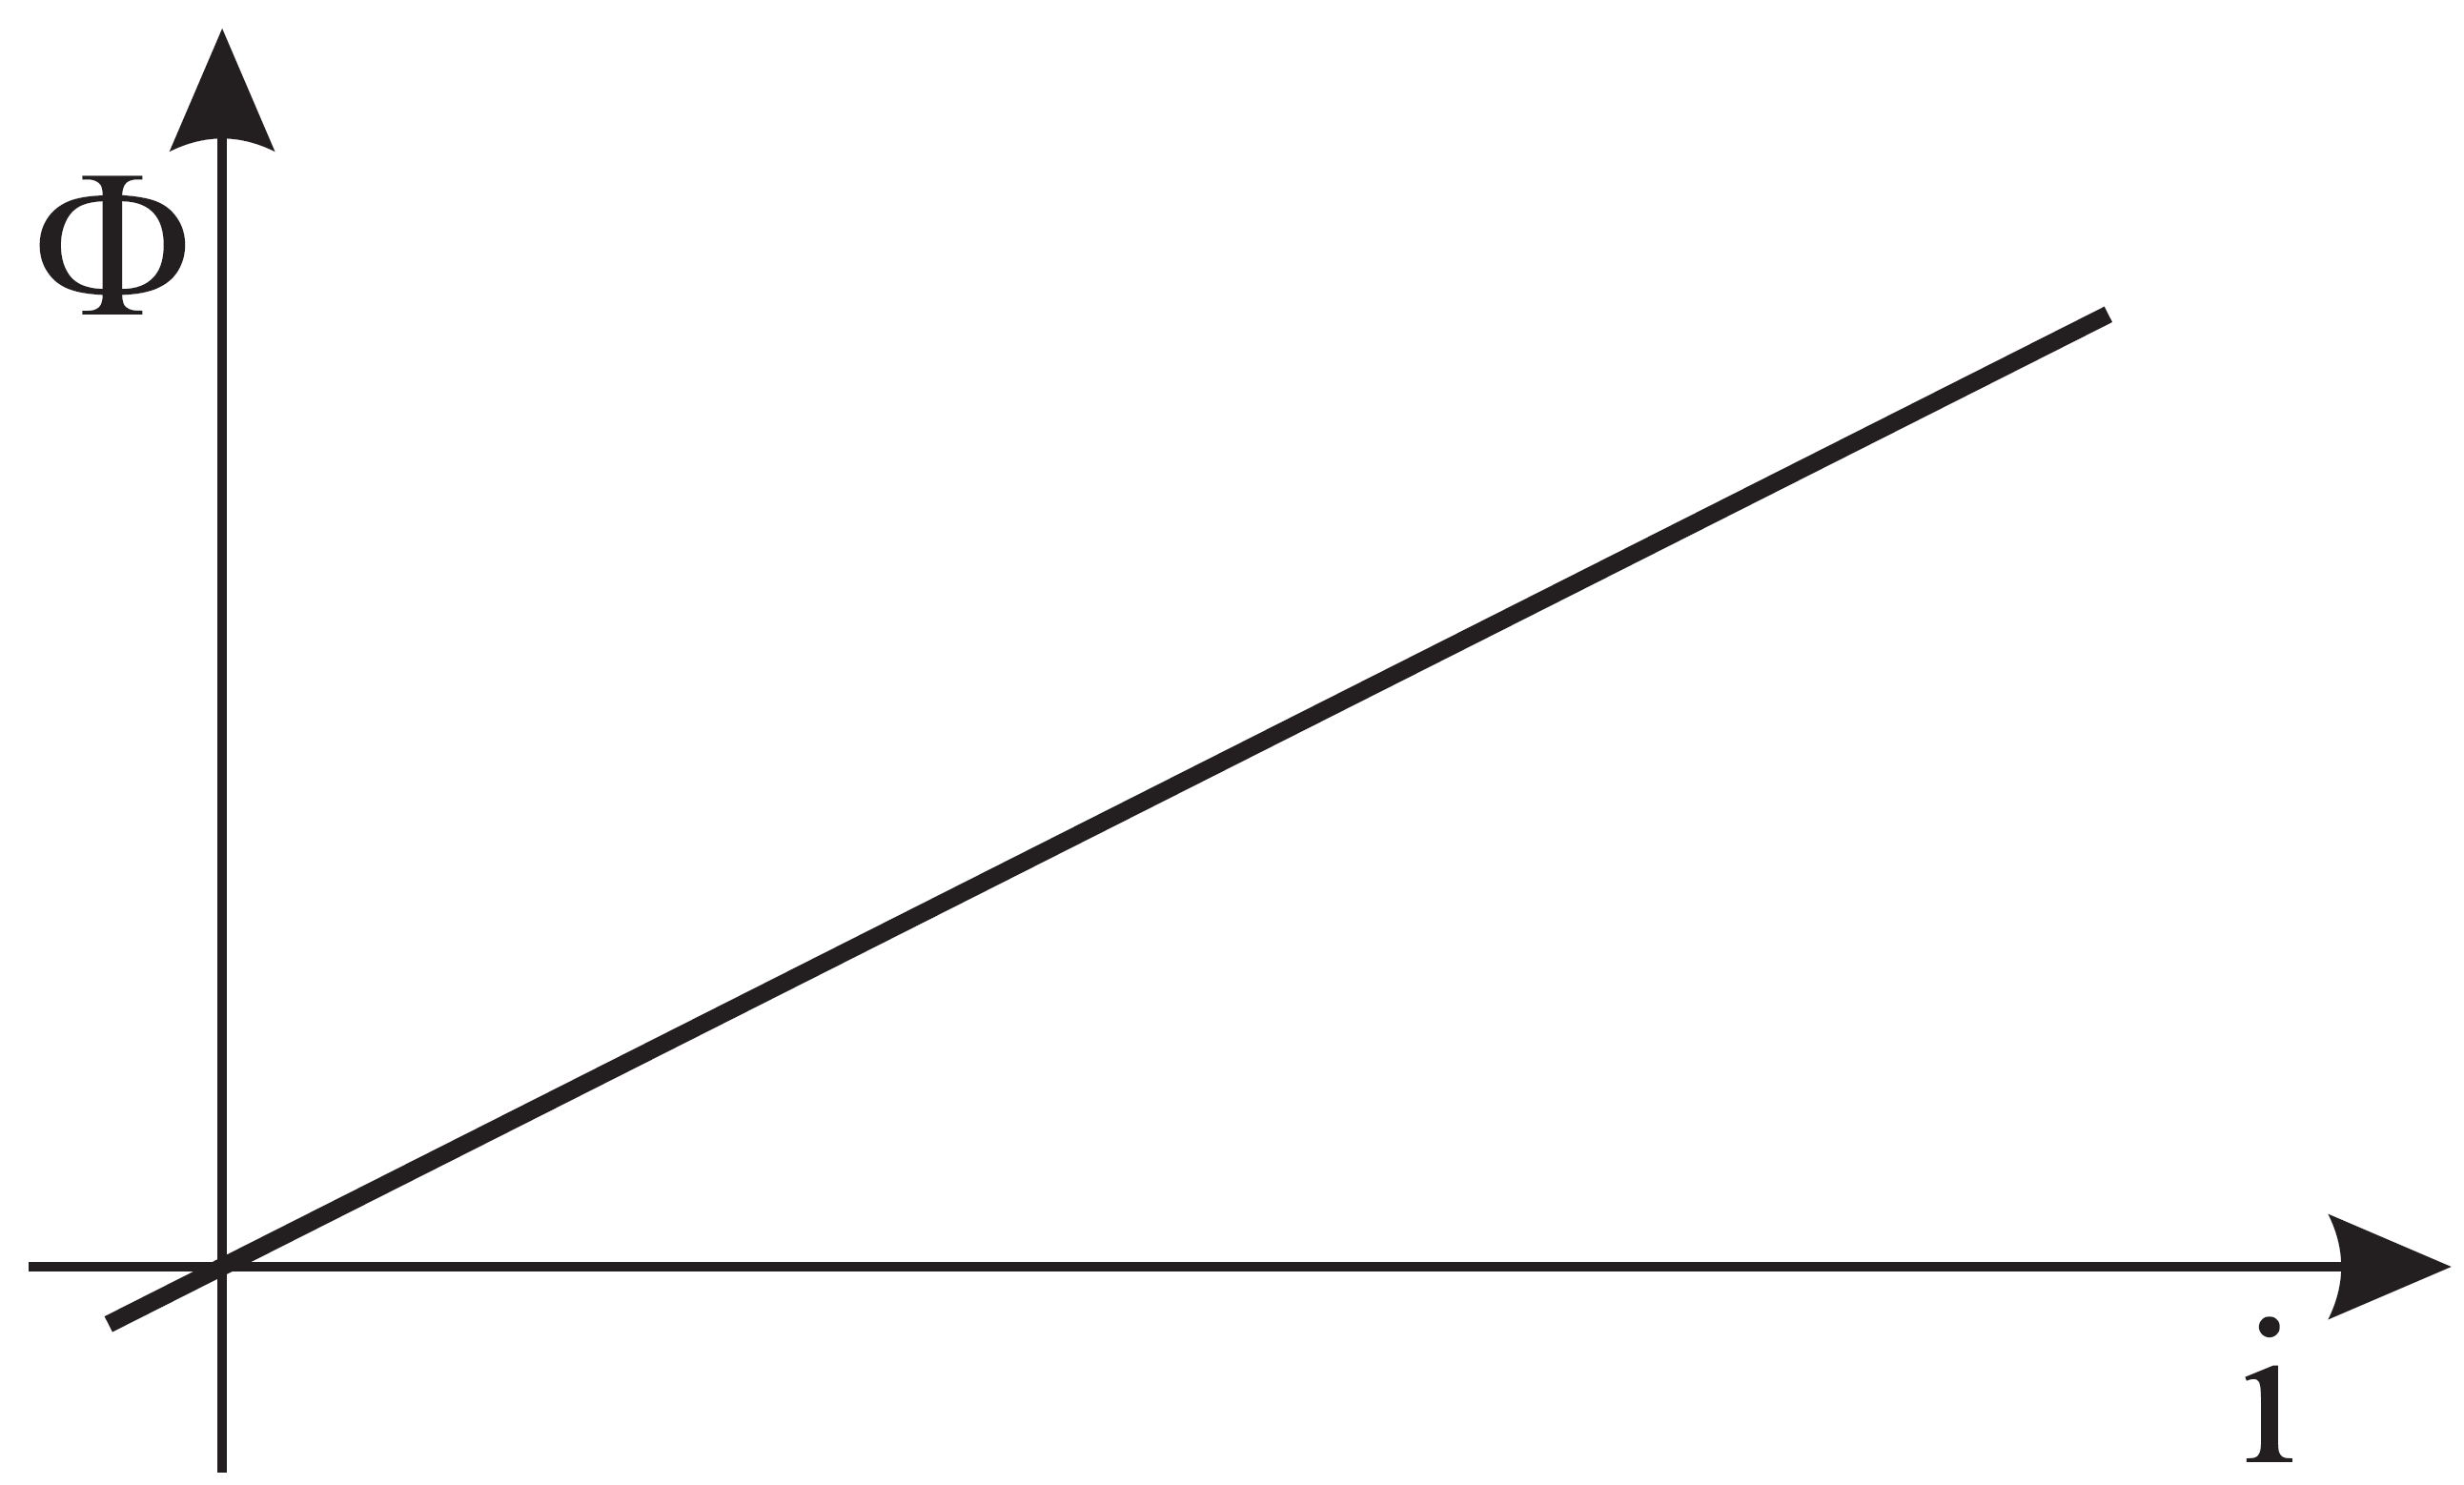
\includegraphics[width=\textwidth]{grundlagen/abb2}
        \caption{Eisen mit gerader Magnetisierungskurve. [$i$ stellt den momentanen Strom dar, von welchem eine umwickelnde Spule durchflossen wird. Dadurch wird im Eisen ein momentaner, magnetischer Fluss $\Phi$ ausgebildet.]}
    \end{minipage}
    \hfill
    \begin{minipage}[b]{0.45\textwidth}
        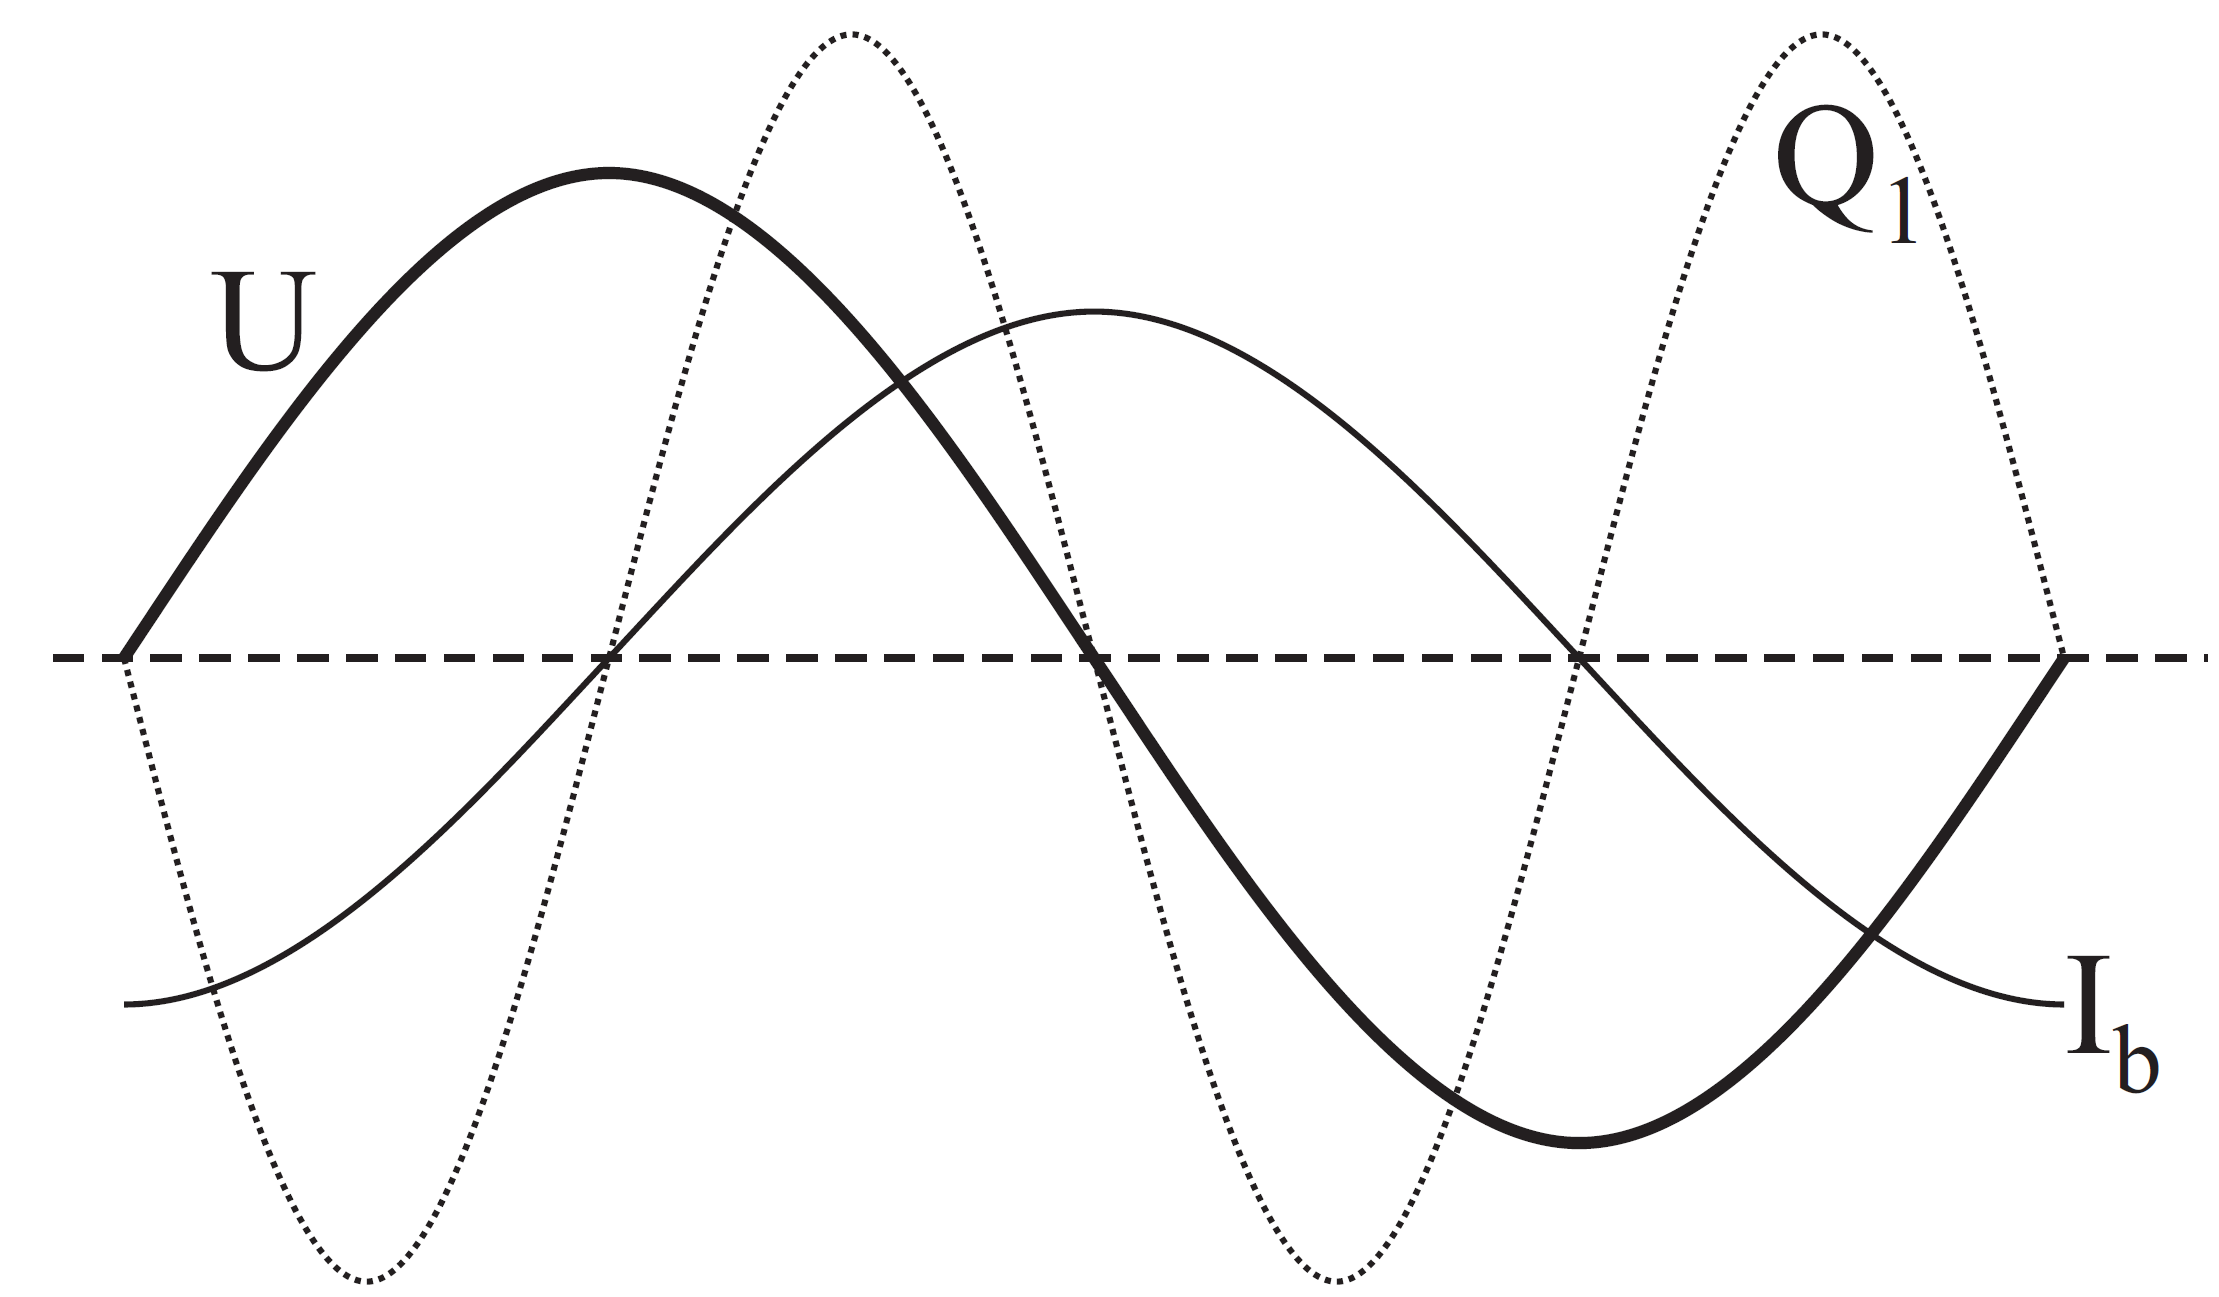
\includegraphics[width=\textwidth]{grundlagen/abb3}
        \caption{Blindleistung $Q_1 = U I_b$. [Verlauf über die Zeit der an einer Spule angelegten Spannung $U$ und dem Magnetisierungsmtrom $I_b$, welcher den Eisenkern in der Spule magnetisiert. Bei einem Magnetisierungsverhalten ohne Hysterese, wie z.B. in Abb. 2, pendelt eine reine Blindleistung $Q_1$ durch die Spule.]}
    \end{minipage}
\end{figure}
Für den Fall, daß die Magnetisierungskurve $\Phi=\Phi(t)$ eine Hysterese aufweist, erhält man den Stromverlauf aus Abb. 4. Dem Netz wird in diesem Fall Leistung entzogen.
\begin{figure}[H]
    \centering
    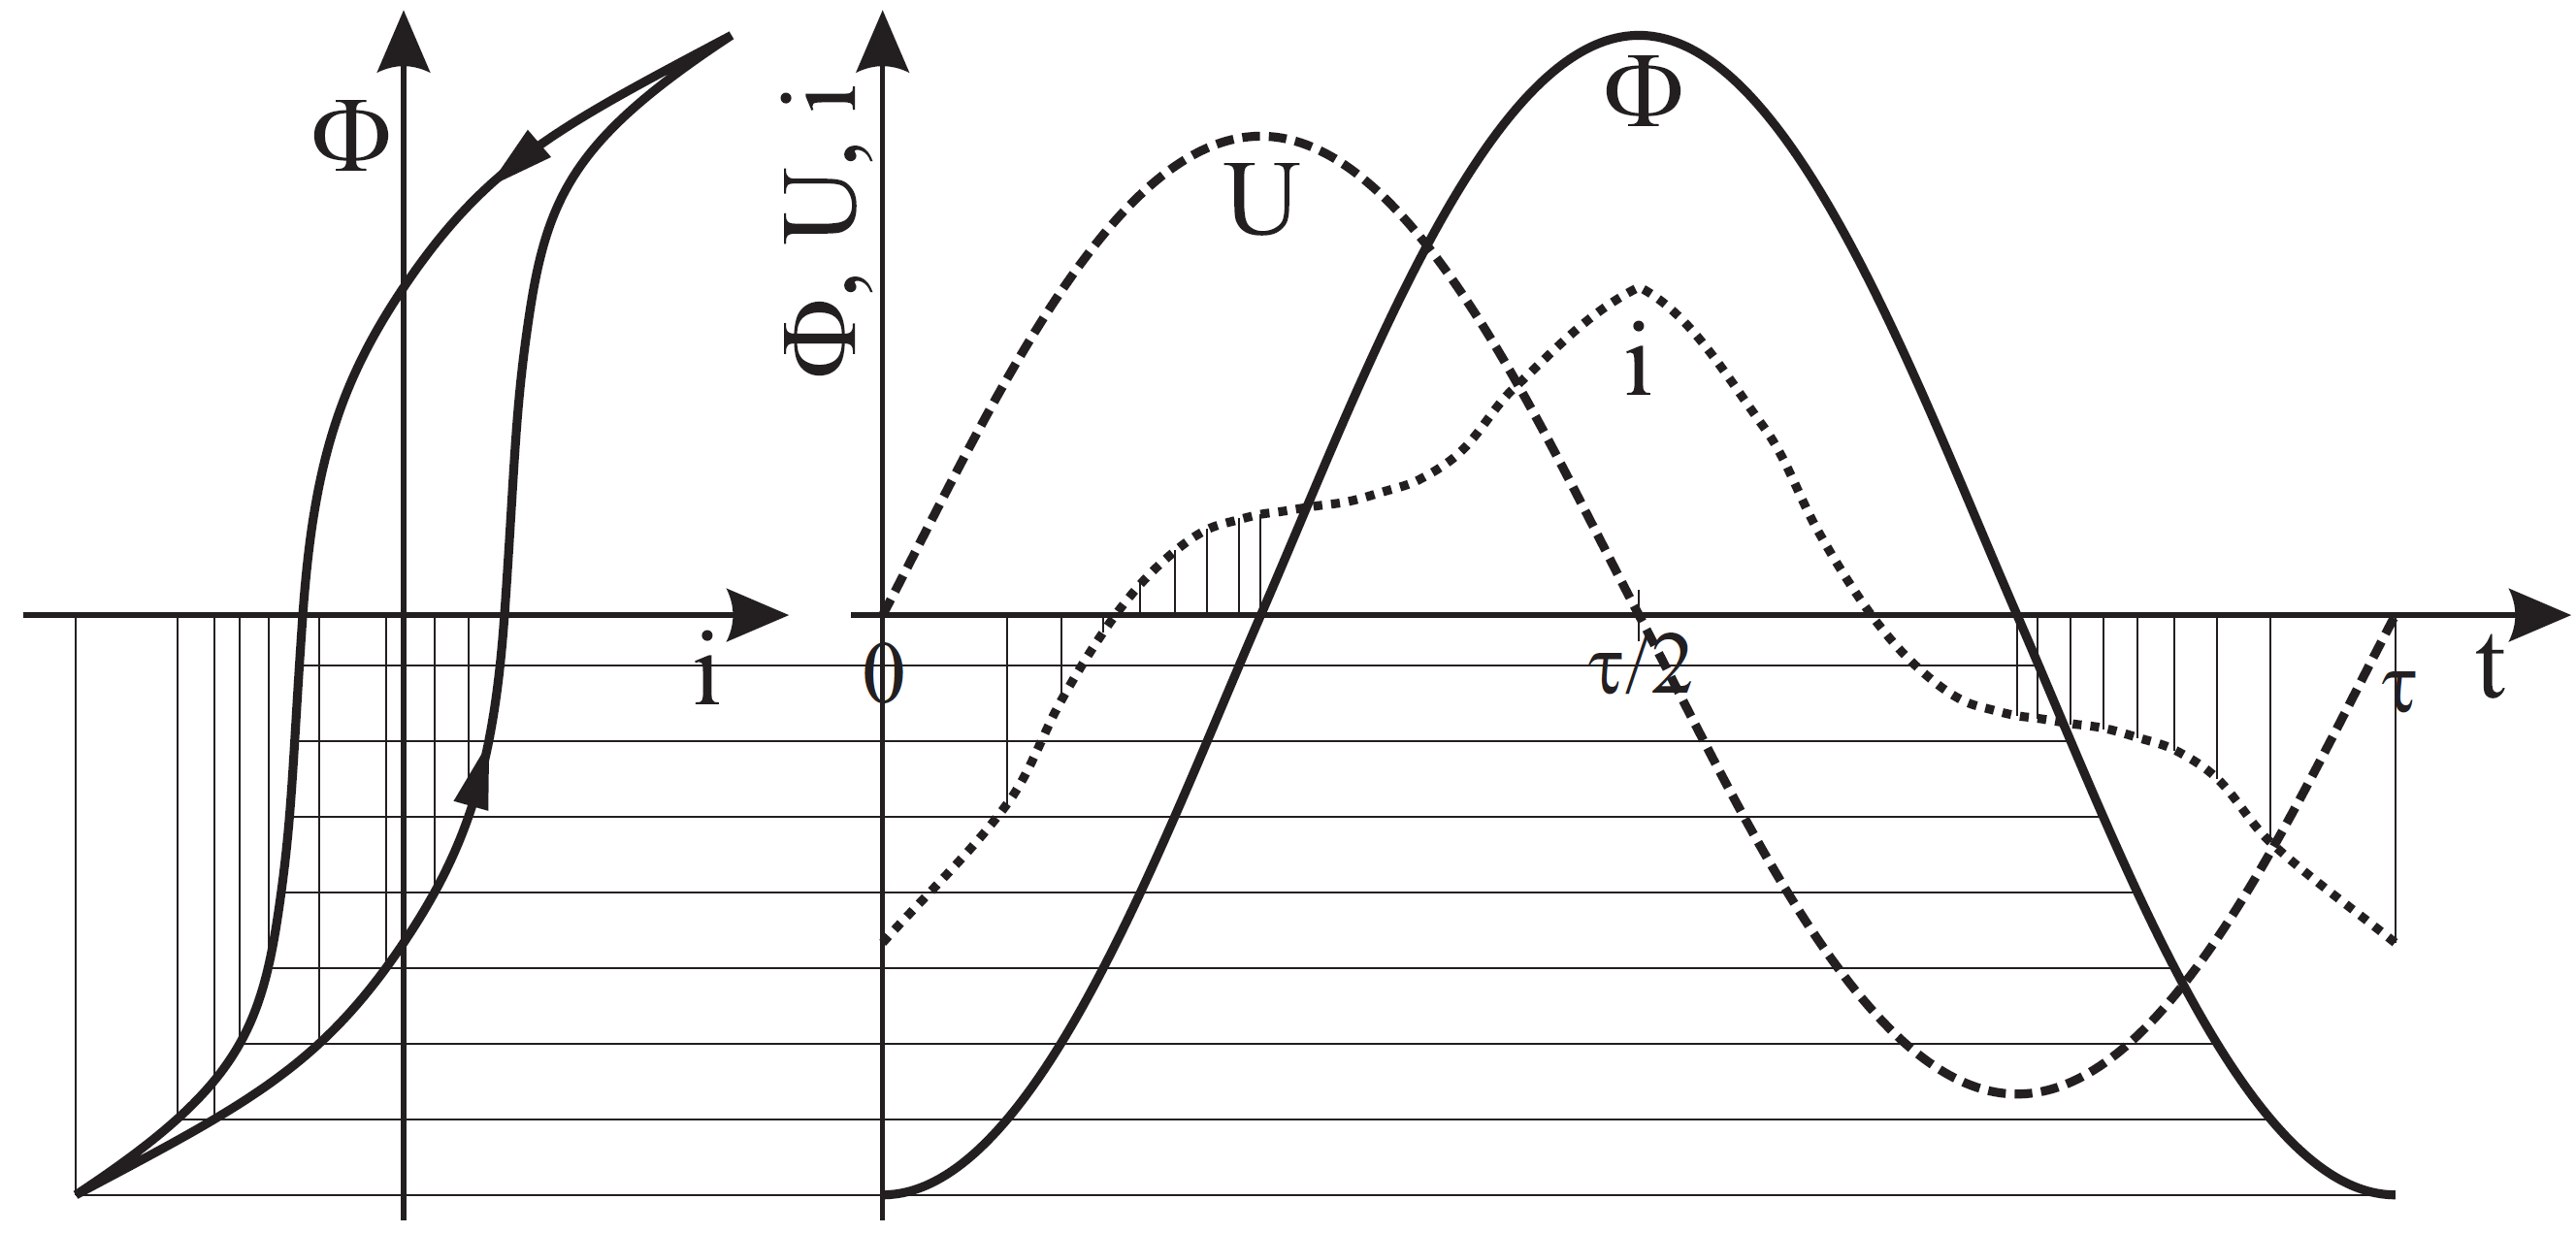
\includegraphics[width=\linewidth/2]{grundlagen/abb4}
    \caption{Spannung $U$, magnetischer Fluß $\Phi$ und Strom $i$ bei Hysterese. [Wie Abb. 2 \& 3, jedoch mit hytsereseartigem Magnetisierungsverhalten.]}
\end{figure}


\subsection{Belastung}

Wird an die Sekundärspule ein Ohm’scher Widerstand $R$ angeschlossen, so fließt auch durch die Sekundärspule ein Strom $I_2$
\begin{equation}
    I_2 = \frac{U_2}{R} = - \frac{n_2}{n_1} \frac{1}{R} U_0 \sin \omega t
\end{equation}
Jede stromdurchflossene Spule erzeugt ein Magnetfeld. Die stromdurchflossene Sekundärspule erzeugt einen von $I_2$ unabhängigen Zusatzfluß $\Phi_2$, der durch die Magnetisierungskurve bestimmt ist. Da der Fluß aber durch Gl. (5) wegen der eingeprägten Netzspannung festgelegt ist, muß $\Phi_2$ kompensiert werden:
\begin{equation}
    \Phi_2 + \Phi_1 = 0
\end{equation}
Diese Kompensation erfolgt durch einen in der Primärspule erzeugten Fluß $\Phi_1$, der durch einen Zusatzstrom $I_{1z}$ zustande kommt. Mit
\begin{equation}
    \Phi_2 = \mu \mu_0 \frac{A}{l} n_2 I_2
\end{equation}
und
\begin{equation}
    \Phi_1 = \mu \mu_0 \frac{A}{l} n_1 I_{1z}
\end{equation}
ergibt sich $I_{1z}$ aus der Bedingung Gl. (9)
\begin{equation}
    I_{1z} = - \frac{n_2}{n_1} I_2
\end{equation}
und wegen Gl. (8):
\begin{equation}
    I_{1z} = \left( \frac{n_2}{n_1} \right)^2 \frac{1}{R} U_1
\end{equation}
Der primäre Zusatzstrom ist bei der angenommenen rein Ohm’schen Belastung in Phase mit der Netzspannung $U_1$. Der durch rein Ohm’sche Belastung der Sekundärseite bewirkte primäre Zusatzstrom $I_{1z}$ verursacht eine Wirkleistungsaufnahme. Das Produkt der $U_1$- und $I_{1z}$-Wellen ist nämlich stets positiv. Selbstverständlich existieren die beiden Ströme $I_b$ und $I_{1z}$ nicht getrennt. Sie setzen sich zu einem Netzstrom $I_1$ zusammen. Dies geschieht, indem man die zu gleichen Zeiten gehörenden Momentanwerte addiert. \\
Eine Sinuswelle entsteht z.B. durch einen mit der Winkelgeschwindigkeit $\omega$ rotierenden Zeiger, wenn man die Spitze des Zeigers in Abhängigkeit vom Winkel $\omega t$ beobachtet (Abb. 5).
\begin{figure}[H]
    \centering
    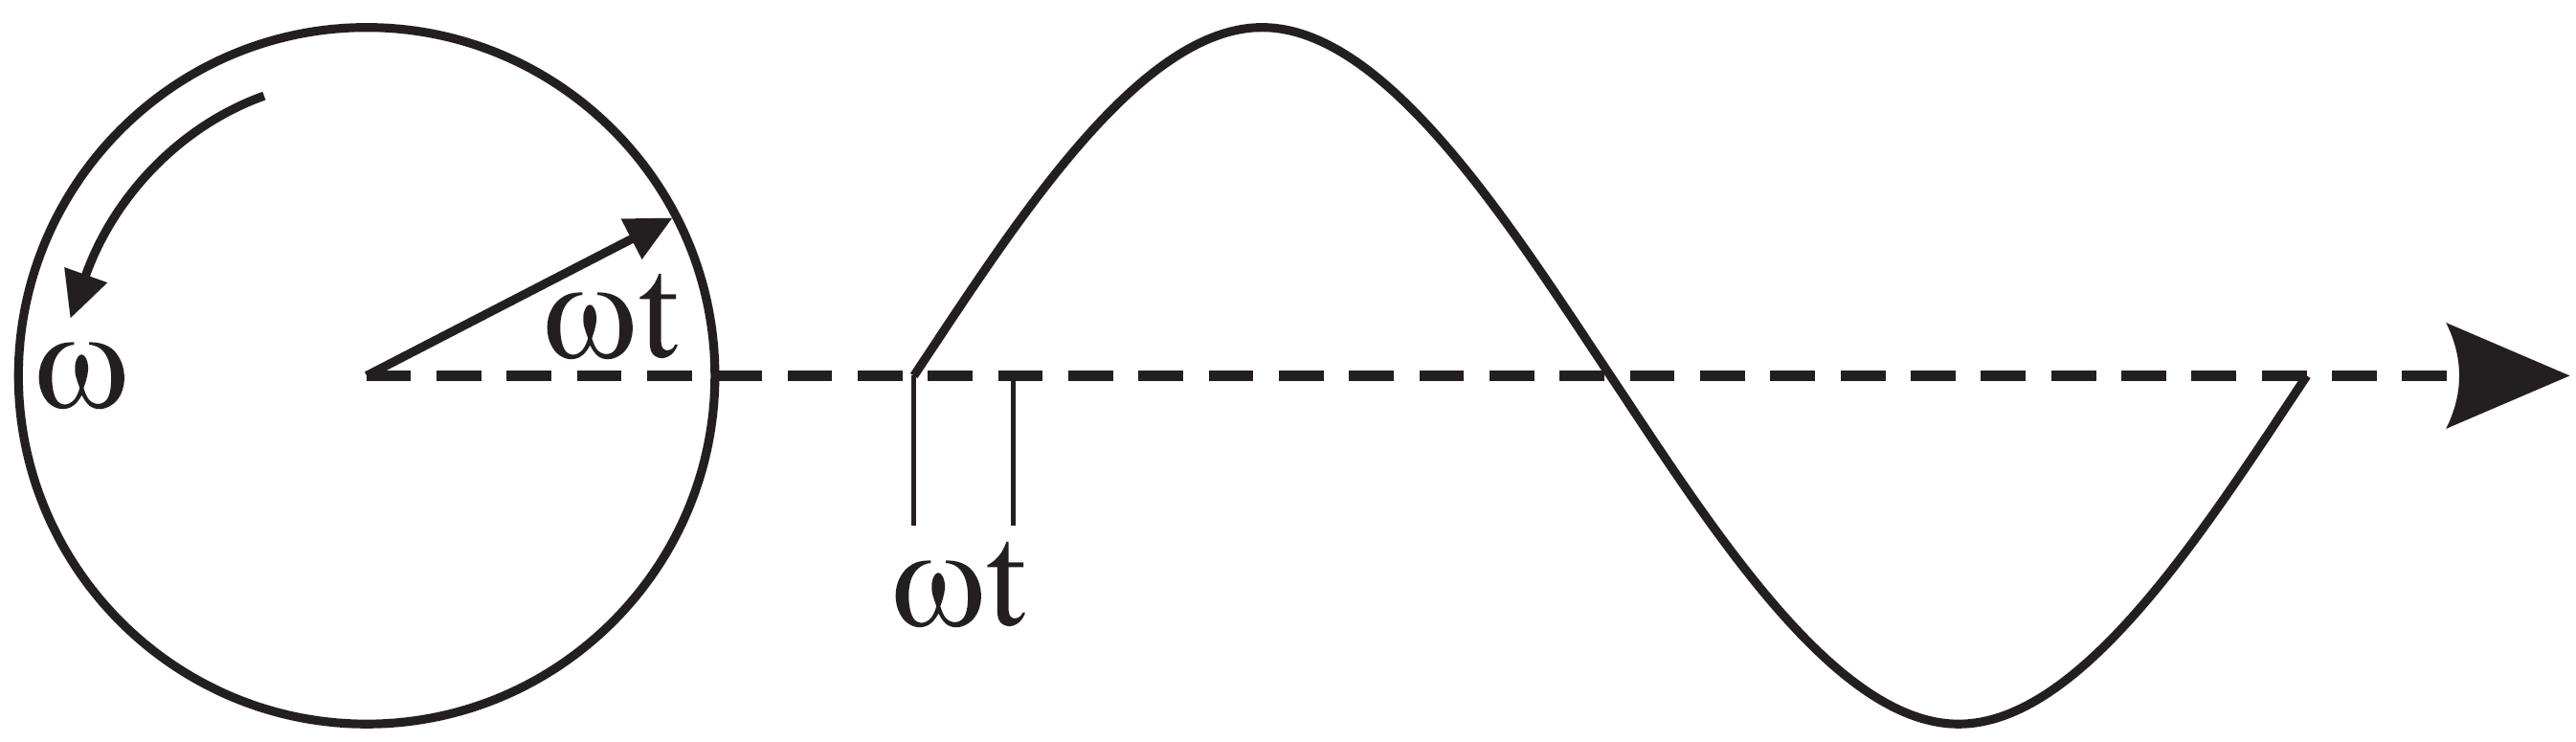
\includegraphics[width=\linewidth/2]{grundlagen/abb5}
    \caption{Zeigerdiagramm und Sinusschwingung. [Zeit $t$ als Laufvariable und Winkelgschwindigkeit $\omega$, mit welcher sich der Zeiger dreht.]}
\end{figure}
Addiert man die Momentanwerte zweier mit gleicher Winkelgeschwindigkeit rotierender Größen, welche gegeneinander eine Phasenverschiebung haben, so setzen sich die Zeiger geometrisch zusammen (Abb. 6). Für den belasteten Transformator zeigt Abb. 7 die Lage der Zeiger. Die Phasenverschiebung $\varphi$ zwischen dem Gesamtstrom $I_1$ (auch Scheinstrom genannt) und der Netzspannung ist nach Abb. 7 gegeben durch:
\begin{figure}[H]
    \centering
    \begin{minipage}[b]{0.3\textwidth}
        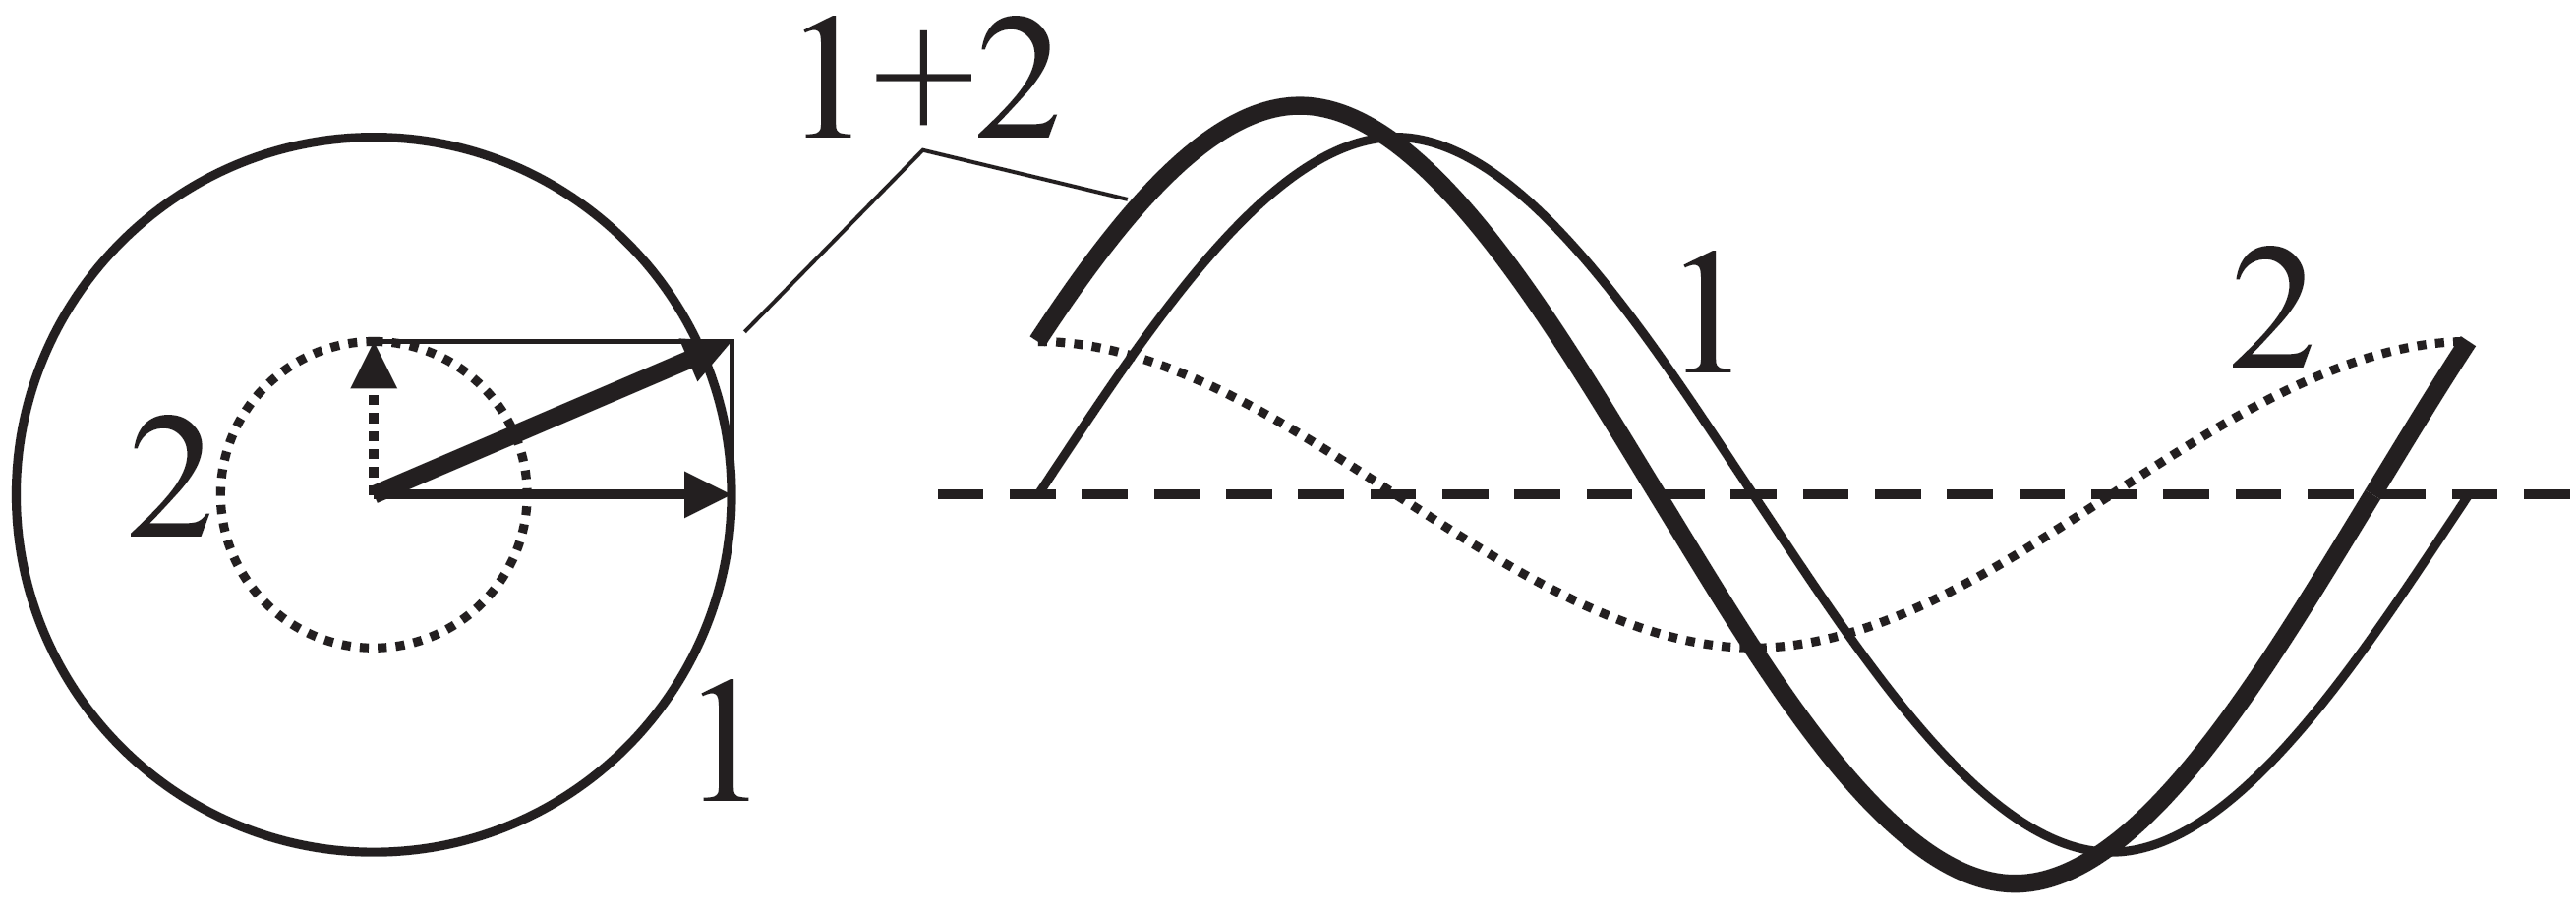
\includegraphics[width=\textwidth]{grundlagen/abb6}
        \caption{Addition zweier Sinusschwingungen. [Überlagerung zweier Wellen wie in Abb. 5 mit \SI{90}{\deg} Phasenverschub.]}
    \end{minipage}
    \hfill
    \begin{minipage}[b]{0.3\textwidth}
        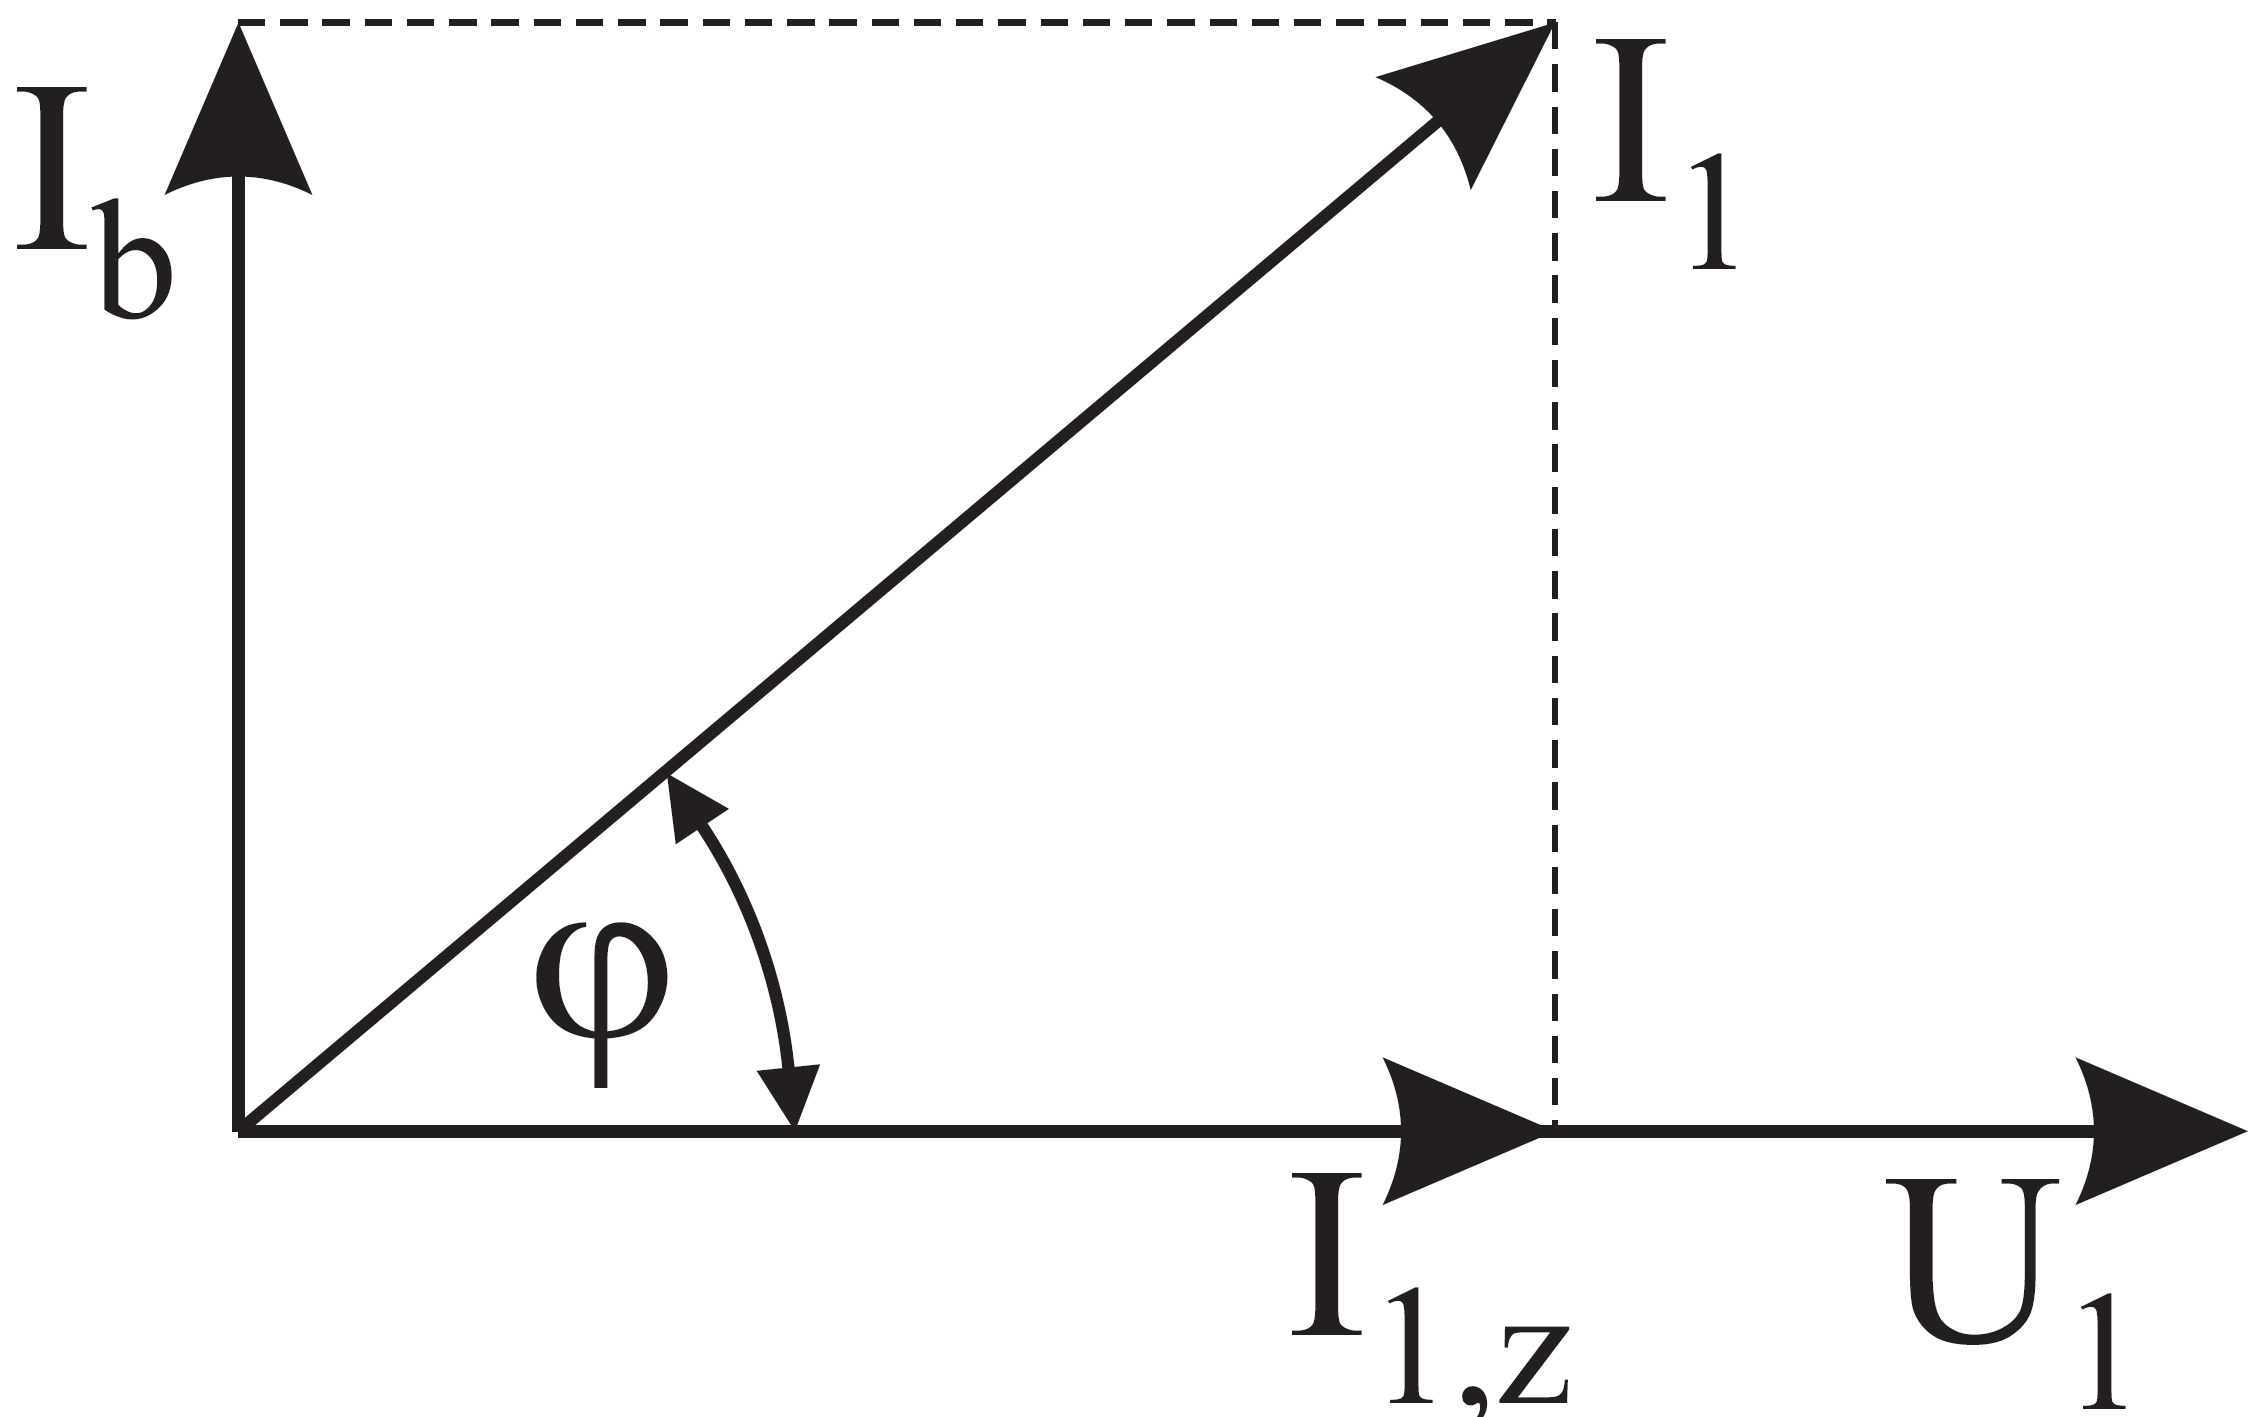
\includegraphics[width=\textwidth]{grundlagen/abb7}
        \caption{Zeigerdiagramm im belasteten Transformator. [$U_1$ ist die angelegte Primärspannung, $I_1$ der insgesamt vom Transformator benötigter Strom, bestehend aus dem zu übertragenden Zusatzstrom $I_{1,z}$ und dem Magnetisierungsstrom $I_b$.]}
    \end{minipage}
    \hfill
    \begin{minipage}[b]{0.3\textwidth}
        \begin{gather}
            \tan \varphi = \frac{I_b}{I_{1z}} \\
            \cos \varphi = \frac{I_{1z}}{I_1} \\
            \sin \varphi = \frac{I_b}{I_1}
        \end{gather}
    \end{minipage}
\end{figure}
Da die Multiplikation der Zähler und Nenner mit $U_1$ an den Verhältnissen Gl. (14) nichts ändert, gilt auch:
\begin{equation}
    \tan \varphi = \frac{Q_1}{P_1} \quad , \quad \cos \varphi = \frac{P_1}{S_1} \quad , \quad \sin \varphi = \frac{Q_1}{S_1}
\end{equation}
Dabei ist $I_{1z} U_1$ die Wirkleistung $P_1$, $I_b U_1$ die Blindleistung $Q_1$ und $I_1 U_1$ die Scheinleistung $S_1$. Bei verlustlosem Transformator muß, damit der Energieerhaltungssatz gewahrt bleibt, die zugeführte Wirkleistung gleich der sekundär abgegebenen Wirkleistung sein:
\begin{equation}
    I_{1z} U_1 = P_1 = P_2 = U_2 I_2
\end{equation}


\subsection{Verluste im Transformator}

Die Spulen des Transformators haben endliche Widerstände: $R_{Sp1}$ und $R_{Sp2}$. Die an ihnen auftretende Wirkleistung
\begin{equation}
    P_{Cu1} = R_{Sp1} I_1^2 \quad , \quad P_{Cu2} = R_{Sp2} I_2^2
\end{equation}
wird als Wärme frei. Ihre Summe $P_{Cu}$ bezeichnet man als Kupferverluste des Transformators.
\begin{equation}
    P_{Cu} = P_{Cu1} + P_{Cu2}
\end{equation}
Außer den Kupferverlusten treten im Transformator auch sogenannte Eisenverluste auf. Sie setzen sich aus den Wirbelstromverlusten und den Hysteresisverlusten zusammen. Die Wirbelstromverluste entstehen durch die elektrische Leitfähigkeit des Eisens. Der Wechselfluß induziert auch im Eisen Spannungen, die sogenannte Wirbelströme hervorrufen, und eine Erwärmung des Eisens bewirken. Durch Unterteilung des Eisenkernes in dünne, gegenseitig isolierte Bleche, kann man das Auftreten von gut leitenden Stromkreisen im Eisen weitgehend verhindern. Die Hysteresisverluste entstehen durch die Abweichung der Eisenmagnetisierung von der Idealform in Abb. 2. Es zeigt sich nämlich, daß nach Zurückgehen des Stromes auf den Wert Null Restmagnetismus (Remanenz) vorhanden ist (Abb. 8). Wird nun in umgekehrter Richtung ein Magnetfeld aufgebracht, so muß erst Energie aufgewendet werden, um das Restfeld abzubauen. Infolge der Transformatorverluste sinkt die Spannung $U_2$ an der Sekundärspule.
\begin{figure}[H]
    \centering
    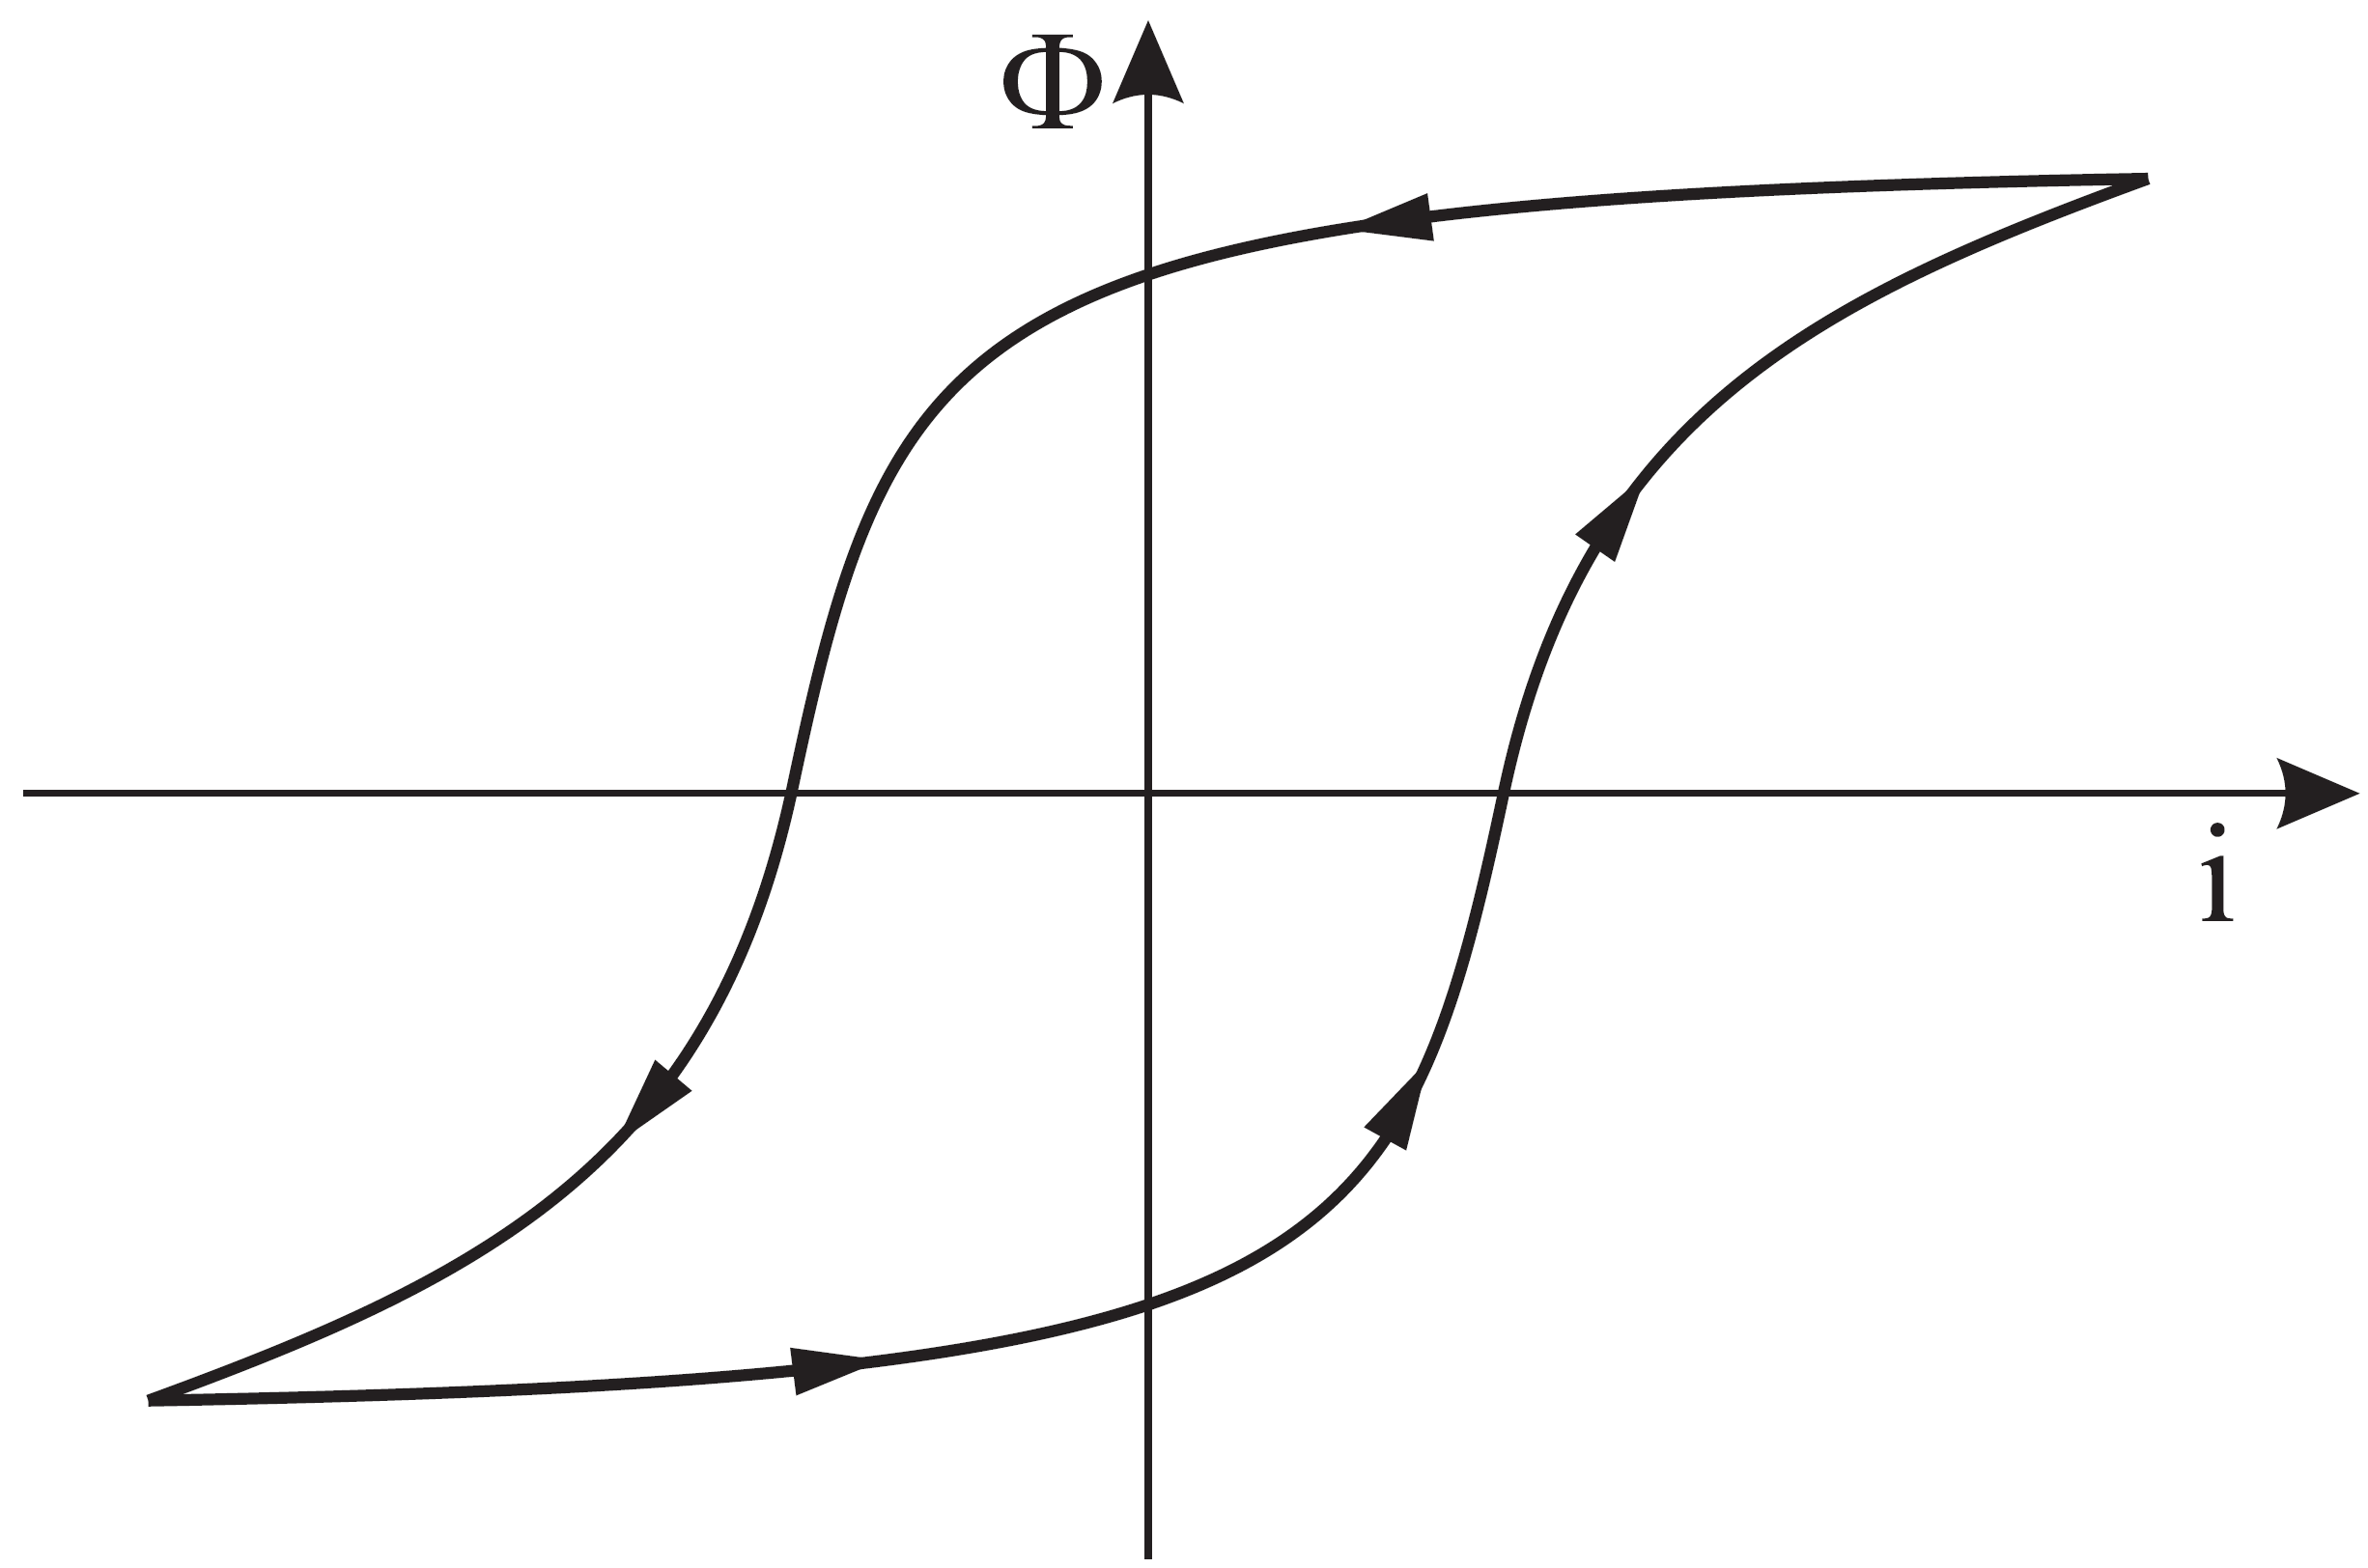
\includegraphics[width=\linewidth/2]{grundlagen/abb8}
    \caption{Hysteresisschleife. [Hystereseschleife wie sie bei realen Materialien wie Eisen vorkommt. $i$ ist der Strom von welchem eine umliegende Spule durchflossen wird, $\Phi$ der magnetische Fluss innerhalb der Spule, im Material. Am Diagramm ist zu erkennen dass, wurde ein Strom angelegt und wieder abgebaut, ein Restfluss (die entsprechende magnetische Flussdichte $B$ wird Remanenz genannt) bestehen bleibt. Um den Fluss $\Phi$ wieder vollständig auf 0 zu bringen, wird ein entgegengesetzter Strom benötigt (die entsprechende Feldstärke wir Koerzitivfeldstärke genannt).]}
\end{figure}
\newpage



\section{Versuchsanordnung}

Ablesungen in Abhängigkeit vom Belastungswiderstand (Last) nach Abb. 9 erlauben es, folgende Größen zu berechnen:
\begin{itemize}
    \item Abgegebene Wirkleistung: $P_2 = U_R I_2$
    \item Aufgenommene Scheinleistung: $S_1 = U_1 I_1$
    \item Phasenverschiebung an der Primärseite: $\cos P_1 / S_1 = P_1 / S_1$, $\varphi = \arccos P_1 / S_1$
    \item Primärer Wirkstrom: $I_{1z} = I_1 \cos \varphi$
    \item Primärer Blindstrom: $I_b = I_1 \sin \varphi = I_1 \sqrt{1 - \cos^2 \varphi}$
    \item Primärer Blindleistung: $Q_1 = I_b U_1$
    \item Verlustleistung: $\Delta P = P_1 - P_2$ als Differenz der zugeführten und der abgegebenen elektrischen Leistung.
    \item Wirkungsgrad: $\eta = N_2 / N_{1w} \cdot \SI{100}{\percent}$ welcher angibt, wieviel Prozent der zugeführten Leistung als elektrische Energie sekundär zur Verfügung steht.
\end{itemize}
\begin{figure}[H]
    \centering
    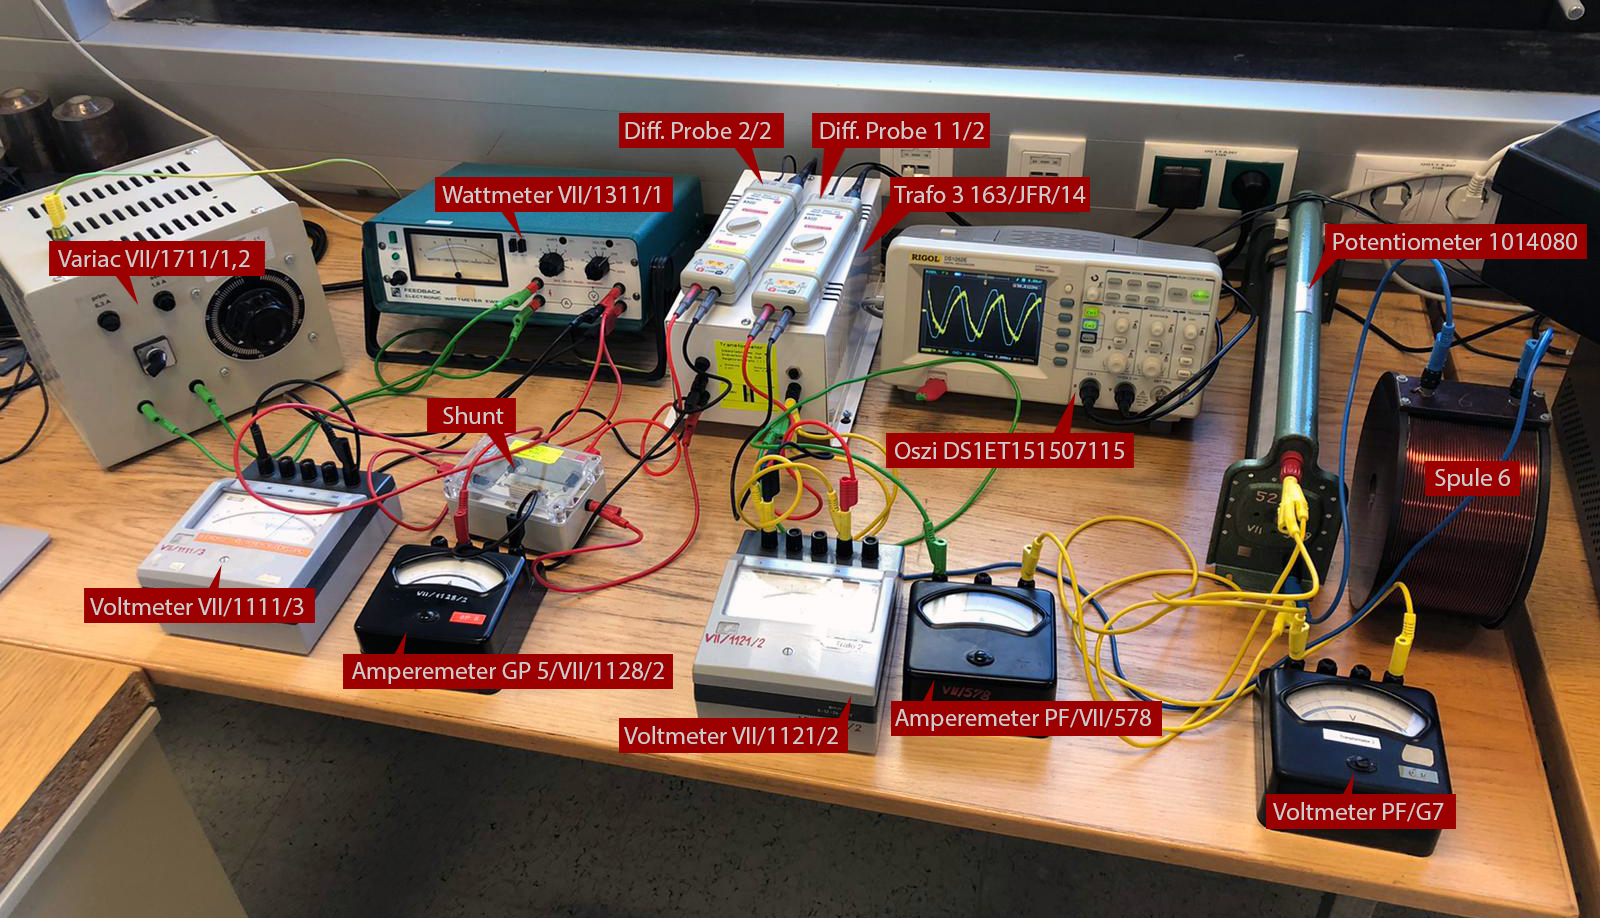
\includegraphics[width=\linewidth]{Trafo-Aufbau.png}
    \caption{Versuchsaufbau - Schaltplan siehe Abb.\ref{fig:Versuchsaufbau_Skizze}}
    \label{fig:Versuchsaufbau}
\end{figure}
\begin{figure}[H]
    \centering
    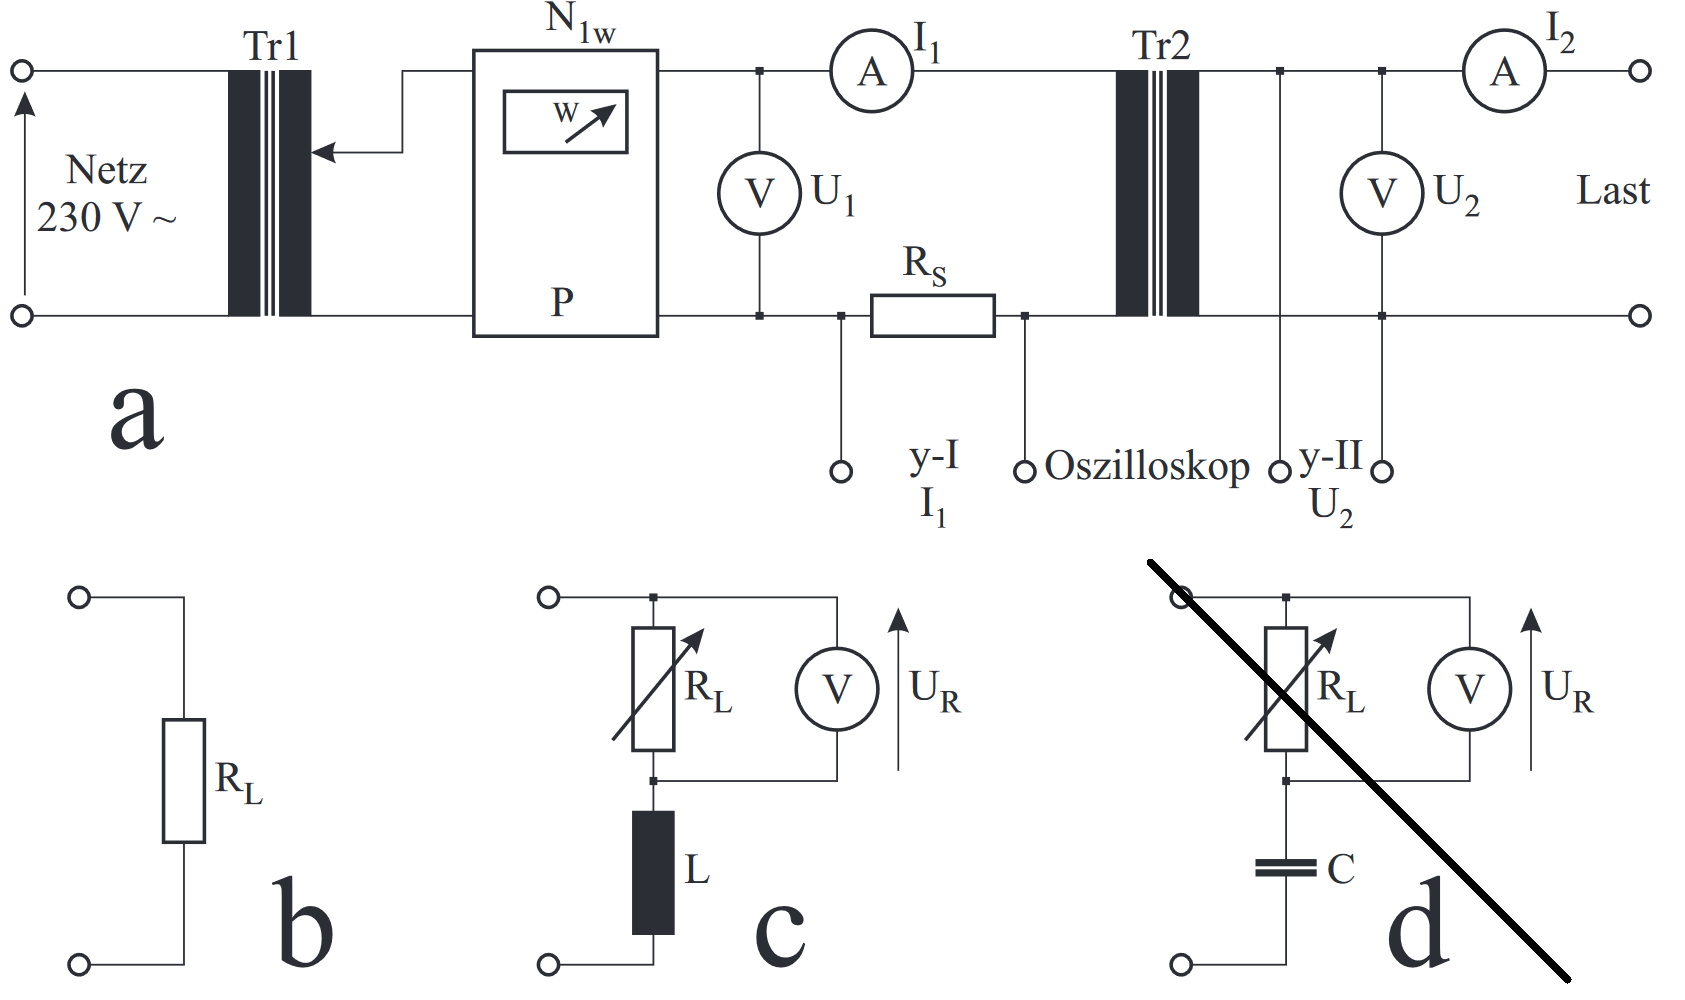
\includegraphics[width=\linewidth]{grundlagen/Versuchsaufbau.PNG}
    \caption{Meßanordnung zur Untersuchung des Transformators Tr2 für a) Leerlauf,b) ohm’sche Last, c) ohm’sche und induktive bzw. \sout{d) ohm’sche und kapazitive Last in Serie}. \\
    \begin{tabular}{ l  l }
        Tr1. . . Variac (RUHSTRAT-VII/1711/1,2)  &   I1. . . Amperemeter (GP 5/VII/1128/2)\\
        Tr2. . . Transformator (163/JFR/14)                  &   U1. . . Voltmeter (VII/111/3) \\
        RS. . . Shunt (ca. 0.5 Ω)           &   I2. . . Amperemeter (PF/VII/578) \\
        RL. . . Potentiometer  (1014080)            &   U2. . . Voltmeter (VII/1121/2) \\
        \sout{C. . . Kondensator}                  &   L. . . Spule\\
        P. . . Wattmeter (VII/1311/1)     &   UR. . . Voltmeter an RL (G7)
    \end{tabular}}
    \label{fig:Versuchsaufbau_Skizze}
\end{figure}
\begin{itemize}
    \item Kupferverluste:
    \begin{itemize}
        \item Primär: $P_{Cu1} = I_1^2 R_{Sp1}$
        \item Sekundär: $P_{Cu2} = I_2^2 R_{Sp2}$
        \item Insgesamt: $P_{Cu} = P_{Cu1} + P_{Cu2}$
    \end{itemize}
    \item Eisenverluste: $P_{Fe} = \Delta P - P_{Cu}$
\end{itemize}
\newpage



\section{Geräteliste}

\begin{table}[H]
    \centering
    \caption{Im Versuch verwendete Geräte und Utensilien.}
    \label{tab:geraete}
    \begin{tabular}{| l | l | l | S C |}
        \hline
        Gerät           & Typ                               & Gerätenummer      & \multicolumn{2}{c|}{Unsicherheit} \\
        \hline
        Variac          & RUHSTRAT                          & VII/1711/1,2      & & \\
        Transformator   & 230V/27V                          & 163/JFR/14        & & \\
        Potentiometer   & $\SI{52}{\ohm} / \SI{3}{\ampere}$ & VII 599 52/3      & & \\
        Spule           &                                   & 6                 & & \\
        Shunt           & $\SI{0,5}{\ohm}$                  &                   & & \\
        Oszilloskop     & Rigol DS1ET151507115              &                   & & \\
        Potentiometer   & Lastwiderstand                    & 1014080           & & \\
        Wattmeter       & Feedback EW604                    & VII/1311/1        & 5 & \si{\percent} \\
        Voltmeter       &                                   & VII/111/3         & 0,5 & \si{\percent} \\
                        &                                   & VII/1121/2        & 0,5 & \si{\percent} \\
                        &                                   & G7                & 0,5 & \si{\percent} \\
        Amperemeter     &                                   & GP 5/VII/1128/2   & 0,5 & \si{\percent} \\
                        &                                   & PF/VII/578        & 1,5 & \si{\percent} \\
        \hline
    \end{tabular}
\end{table}



\section{Versuchsdurchführung \& Messergebnisse}

Die Experimentatoren führen deren Teile des Versuches (Angermann: Leerlauf \& ohm'sche Last, Gössl: ohm'sch-induktive Last) aufgrund der zum Zeitpunkt der Durchführung geltenden Lockdown-Richtlinien zeitlich getrennt durch. \\
Alle komplexen Wechselstromgrößen sind in Effektivwerten angegeben. \\
Wenn nicht anderes angegeben werden die Messbereiche der Messgeräte zur bestmöglichen Genauigkeit eingestellt.
\begin{table}[H]
    \centering
    \caption{Die an den Messgeräten eingestellten Messbereiche zur Berechnung der absoluten Unsicherheiten.}
    \label{tab:skala}
    \begin{tabular}{| l | *{6}{S|}}
        \hline
        Größe                   & {$P_1 \ / \ \si{\watt}$}  & {$U_1 \ / \ \si{\volt}$}  & {$I_1 \ / \ \si{\milli\ampere}$}  & {$U_2 \ / \ \si{\volt}$}  & {$I_2 \ / \ \si{\milli\ampere}$}    & {$U_R \ / \ \si{\volt}$} \\
        \hline
        Leerlauf                & 40                        & 240                       & 120                               & 24                        &                                         & \\
        Ohm'sche Last           & 40                        & 240                       & 600                               & 24                        & 1000                                     & \\
        Ohm'sch-induktive Last  & 40                        & 240                       & 600                               & 24                        & 1000                                     & 30 \\
        \hline
    \end{tabular}
\end{table}

Die Versuchsanordnung wird Abb. \ref{fig:Versuchsaufbau_Skizze} a entsprechend aufgebaut, unter Spannung gesetzt und die Messwerte werden in Tab. \ref{tab:durchalles} notiert. \\

Die ohm'sche Last $R$ wird lt. Abb. \ref{fig:Versuchsaufbau_Skizze} b in die Anordnung eingesetzt, welche wieder unter Spannung gesetzt wird und die Messwerte werden ebenfalls in Tab. \ref{tab:durchalles} hinzugefügt. \\

Von Sebastian Gössl wird die bestehende Anordnung weiterverwendet und nur die Spule $L$ lt. Abb. \ref{fig:Versuchsaufbau_Skizze} c zur ohm'schen Last hinzugefügt. Der Aufbau wird unter Spannung gesetzt und das Potentiometer wird schrittweise verstellt, wobei jedes Mal der Sekundärstrom $I_2$ und der Spannungsabfall $U_R$ am Widerstand $R$ in Tab. \ref{tab:durchleistung} notiert wird.
\begin{table}[H]
    \centering
    \caption{Gemessener Sekundärstrom $I_2$ und der Spannungsabfall $U_R$ bei unterschiedlichen Potentiometerstellungen. Die hervorgehobene Messung 12 zeigt die in Tab. \ref{tab:auswleistung} gefundene Potentiometerstellung mit der höchsten Wirkleistung $P_2$. \\
    $I_2$ \dots Sekundärstrom $\Delta I_2=\SI{5}{\milli\ampere}$ \\
    $U_R$ \dots Spannungsabfall am Widerstand $R$ $\Delta U_R=\SI{0,15}{\volt}$}
    \label{tab:durchleistung}
    \begin{tabular}{| l | *{2}{S|}}
        \hline
        Messung & {$I_2 \ / \ \si{\milli\ampere}$}  & {$U_R \ / \ \si{\volt}$} \\
        \hline
         1      & 330                               & 17,00 \\
         2      & 340                               & 16,75 \\
         3      & 350                               & 16,50 \\
         4      & 360                               & 16,25 \\
         5      & 360                               & 16,25 \\
         6      & 370                               & 16,00 \\
         7      & 380                               & 15,75 \\
         8      & 380                               & 15,50 \\
         9      & 390                               & 15,25 \\
        10      & 400                               & 15,00 \\
        11      & 410                               & 14,75 \\
        \hline
        12      & 420                               & 14,50 \\
        \hline
        13      & 430                               & 14,00 \\
        14      & 440                               & 13,50 \\
        15      & 450                               & 13,00 \\
        16      & 460                               & 12,75 \\
        17      & 480                               & 12,00 \\
        18      & 490                               & 11,75 \\
        19      & 500                               & 11,00 \\
        20      & 510                               & 10,75 \\
        21      & 530                               & 10,00 \\
        22      & 540                               &  9,25 \\
        23      & 560                               &  8,25 \\
        24      & 570                               &  7,50 \\
        25      & 580                               &  7,00 \\
        26      & 590                               &  6,00 \\
        27      & 600                               &  5,50 \\
        28      & 600                               &  4,50 \\
        29      & 620                               &  4,00 \\
        30      & 620                               &  3,50 \\
        \hline
    \end{tabular}
\end{table}
Mit den Werten aus Tab. \ref{tab:durchleistung} wird die Potentiometerstellung, bei welcher die am Widerstand $R$ verbrauchte Leistung $P_2$ (sekundäre Wirkleistung, ohm'scher Widerstand der Spule vernachlässigt) maximal wird, ermittelt. Diese Auswertung wird vor dem nächsten Schritt (Messung aller geforderten Werte) durchgeführt, aber erst im \hyperref[sec:auswertung]{Kapitel Auswertung} in Tab. \ref{tab:auswleistung} angeführt. \\
Das Maximum von $P_2$ befindet sich lt. Tab. \ref{tab:auswleistung} bei Messung 12 mit $R=\SI{34,5+-0,8}{\ohm}, \ P_2=\SI{6,09+-0,14}{\watt}$. Die Potentiometerstellung wird wieder gefunden indem es verschoben wird bis wieder gleiche Werte für $I_2=\SI{420+-5}{\milli\ampere}$ und $U_R=\SI{14,50+-0,15}{\volt}$ erreicht werden. Anschließend werden alle anderen Messwerte abgelesen und in Tab. \ref{tab:durchalles} eingetragen.
\begin{table}[H]
    \centering
    \caption{Messwerte der Versuche. Die Unsicherheiten ergeben sich aus den relativen Unsicherheiten in Tab. \ref{tab:geraete} und den Messbereichen in Tab. \ref{tab:skala}. \\
    $U_1$ \dots Primärspannung \\
    $I_1$ \dots Primärstrom \\
    $P_1$ \dots Primärleistung \\
    $U_2$ \dots Sekundärspannung \\
    $I_2$ \dots Sekundärstrom \\
    $U_R$ \dots Spannungsabfall am Widerstand}
    \label{tab:durchalles}
    \begin{tabular}{| l | *{3}{SS|}}
        \hline
        Versuch             & \multicolumn{2}{C|}{U_1 \ / \ \si{\volt}} & \multicolumn{2}{C|}{I_1 \ / \ \si{\milli\ampere}} & \multicolumn{2}{C|}{P_1 \ / \ \si{\watt}} \\
        \hline
        Leerlauf            & 160,0 & +-1,2                             & 110,0 & +-1,8                                     & 9,0   & +-2,0 \\
        Ohm'sch             & 160,0 & +-1,2                             & 170   & +-9                                       & 24,8  & +-2,0 \\
        Ohm'sch-Induktiv    & 162,0 & +-1,2                             & 160   & +-9                                       & 16,2  & +-2,0 \\
        \hline
        \hline
        Versuch             & \multicolumn{2}{C|}{U_2 \ / \ \si{\volt}} & \multicolumn{2}{C|}{I_2 \ / \ \si{\milli\ampere}} & \multicolumn{2}{C|}{U_R \ / \ \si{\volt}} \\
                            \hline
        Leerlauf            & 21,20 & +-0,12                            &   0   &                                           &       & \\
        Ohm'sch             & 21,00 & +-0,12                            & 760   & +-5                                       &       & \\
        Ohm'sch-Induktiv    & 21,40 & +-0,12                            & 420   & +-5                                       & 14,50 & +-0,15 \\
        \hline
    \end{tabular}
\end{table}
\begin{figure}[H]
    \centering
    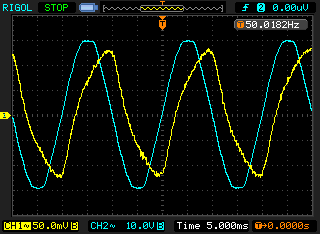
\includegraphics[width=\linewidth/2]{oszi}
    \caption{Oszilloskopaufnahme bei maximaler Leistung am Widerstand beim LR-Versuch. Kanal 1 (gelb): Spannungsabfall am Shunt $\propto$ Primärstrom $i_1(t)$, Kanal 2 (blau): Sekundärspannung $u_2(t)$. Angeschlossen wie in Abb. \ref{fig:Versuchsaufbau_Skizze} eingezeichnet.}
    \label{fig:oszi}
\end{figure}



\section{Auswertung}
\label{sec:auswertung}

In der Auswertung werden zur erhöhten Genauigkeit durchgehend ungerundete Werte bis zu den Endergebnissen verwendet und nur zur Darstellung gerundet. Daher ist es erforderlich, dass dies auch bei einer erneuten Auswertung geschieht. \\
Zur Berechnung der Unsicherheiten wird, wenn nicht anders angegeben, die Größtunsicherheitsmethode verwendet.


\subsection{Leistungsmaximum}

Mit den Werten aus Tab. \ref{tab:durchleistung} wird der Widerstandswert $R$ des Potentiometers $R$ und die sekundäre Wirkleistung $P_2$ berechnet und sowohl in Tab. \ref{tab:auswleistung} als auch Abb. \ref{fig:auswleistung} gegeneinander aufgeführt.
\begin{equation}
\begin{aligned}
    R &= \frac{U_R}{I_2}    &\qquad \Delta R &= R \left( \frac{\Delta U_R}{U_R} + \frac{\Delta I_2}{I_2} \right) \\
    P_2 &= U_R I_2          &\qquad \Delta P_2 &= P_2 \left( \frac{\Delta U_R}{U_R} + \frac{\Delta I_2}{I_2} \right)
    \label{eq:auswleistung}
\end{aligned}
\end{equation}
\begin{table}[H]
    \centering
    \caption{Mit den Werten aus Tab. \ref{tab:durchleistung} berechneter Widerstandswert $R$ des Potentiometers $R$ und sekundäre Wirkleistung $P_2$ lt. Glg. \ref{eq:auswleistung}, mit ihrem Maximum bei der hervorgehobenen Messung 12. \\
    $R$ \dots Widerstandswert des Potentiometers $R$ \\
    $P_2$ \dots sekundäre Wirkleistung}
    \label{tab:auswleistung}
    \begin{tabular}{| l | *{2}{S|}}
        \hline
        Messung & {$R \ / \ \si{\ohm}$} & {$P_2 \ / \ \si{\watt}$} \\
        \hline
         1      & 51,5 +- 1,3           & 5,61 +- 0,14 \\
         2      & 49,3 +- 1,2           & 5,70 +- 0,14 \\
         3      & 47,1 +- 1,2           & 5,78 +- 0,14 \\
         4      & 45,1 +- 1,1           & 5,85 +- 0,14 \\
         5      & 45,1 +- 1,1           & 5,85 +- 0,14 \\
         6      & 43,2 +- 1,0           & 5,92 +- 0,14 \\
         7      & 41,4 +- 1,0           & 5,99 +- 0,14 \\
         8      & 40,8 +- 1,0           & 5,89 +- 0,14 \\
         9      & 39,1 +- 0,9           & 5,95 +- 0,14 \\
        10      & 37,5 +- 0,9           & 6,00 +- 0,14 \\
        11      & 36,0 +- 0,9           & 6,05 +- 0,14 \\
        \hline
        12      & 34,5 +- 0,8           & 6,09 +- 0,14 \\
        \hline
        13      & 32,6 +- 0,8           & 6,02 +- 0,14 \\
        14      & 30,7 +- 0,7           & 5,94 +- 0,14 \\
        15      & 28,9 +- 0,7           & 5,85 +- 0,14 \\
        16      & 27,7 +- 0,7           & 5,87 +- 0,14 \\
        17      & 25,0 +- 0,6           & 5,76 +- 0,14 \\
        18      & 24,0 +- 0,6           & 5,76 +- 0,14 \\
        19      & 22,0 +- 0,6           & 5,50 +- 0,13 \\
        20      & 21,1 +- 0,6           & 5,48 +- 0,14 \\
        21      & 18,9 +- 0,5           & 5,30 +- 0,13 \\
        22      & 17,1 +- 0,5           & 5,00 +- 0,13 \\
        23      & 14,7 +- 0,4           & 4,62 +- 0,13 \\
        24      & 13,2 +- 0,4           & 4,28 +- 0,13 \\
        25      & 12,1 +- 0,4           & 4,06 +- 0,13 \\
        26      & 10,2 +- 0,4           & 3,54 +- 0,12 \\
        27      &  9,2 +- 0,4           & 3,30 +- 0,12 \\
        28      &  7,5 +- 0,4           & 2,70 +- 0,12 \\
        29      &  6,5 +- 0,3           & 2,48 +- 0,12 \\
        30      &  5,6 +- 0,3           & 2,17 +- 0,12 \\
        \hline
    \end{tabular}
\end{table}


\subsection{Hauptaufgabe}

Mit den gemessenen Werten in Tab. \ref{tab:durchalles} werden die in Tab. \ref{tab:aufgabe} geforderten Werte (Formeln hier in Glg. \ref{eq:ausw} erneut mit Unsicherheitsberechnung angegeben) berechnet und in Tab. \ref{tab:auswalles} aufgelistet. Bei der ohm'sch-induktiven Last muss darauf geachtet werden, dass für die Berechnung der sekundären Wirkleistung $P_2$ der Spannungsabfall am Widerstand $R$ verwendet wird, da man ansonsten die sekundäre Scheinleistung $S_2$ erhalten würde.
\begin{equation}
\begin{aligned}
    S_1 &= U_1 I_1                              &\qquad \Delta S_1 &= S_1 \left( \frac{\Delta U_1}{U_1} + \frac{\Delta I_1}{I_1} \right) \\
    Q_1 &= \sqrt{S_1^2 - P_1^2}                 &\qquad \Delta Q_1 &= \frac{1}{Q_1} \left( S_1 \Delta S_1 + P_1 \Delta P_1 \right) \\
    \cos \phi &= \frac{P_1}{S_1}                &\qquad \Delta \cos \phi &= \cos \phi \left( \frac{\Delta P_1}{P_1} + \frac{\Delta S_1}{S_1} \right) \\
    P_2 &= U_2 I_2 \ (\text{bzw.} \ U_R I_2)    &\qquad \Delta P_2 &= P_2 \left( \frac{\Delta U_2}{U_2} + \frac{I_2}{I_2} \right) \\
    P_V &= P_1 - P_2                            &\qquad \Delta P_V &= \Delta P_1 + \Delta P_2 \\
    \eta &= \frac{P_2}{P_1}                     &\qquad \Delta \eta &= \eta \left( \frac{\Delta P_2}{P_2} + \frac{\Delta P_1}{P_1} \right)
    \label{eq:ausw}
\end{aligned}
\end{equation}
\begin{table}[H]
    \centering
    \caption{Mit den Werten aus Tab. \ref{tab:durchalles} lt. Glg. \ref{eq:ausw} berechnete Werte.}
    \label{tab:auswalles}
    \begin{tabular}{| l | *{3}{SS|}}
        \hline
        Versuch             & \multicolumn{2}{C|}{S_1 \ / \ \si{\va}}   & \multicolumn{2}{C|}{Q_1 \ / \ \si{\var}}  & \multicolumn{2}{C|}{\cos \phi \ / \ 1} \\
        \hline
        Leerlauf            & 17,6  & +-0,5                             & 15,1  & +-1,8                             & 0,51  & +-0,13 \\
        Ohm'sch             & 27,2  & +-1,7                             & 11    & +-9                               & 0,91  & +-0,14 \\
        Ohm'sch-Induktiv    & 25,9  & +-1,7                             & 20    & +-4                               & 0,63  & +-0,12 \\
        \hline
        \hline
        Versuch             & \multicolumn{2}{C|}{P_2 \ / \ \si{\watt}} & \multicolumn{2}{C|}{P_V \ / \ \si{\watt}} & \multicolumn{2}{C|}{\eta \ / \ \si{\percent}} \\
                            \hline
        Leerlauf            &  0    &                                   & 9,0   & +-2,0                             & 0     & \\
        Ohm'sch             & 15,96 & +-0,20                            & 8,8   & +-2,2                             & 0,64  & +-0,06 \\
        Ohm'sch-Induktiv    &  6,09 & +-0,11                            & 10,1  & +-2,2                             & 0,38  & +-0,06 \\
        \hline
    \end{tabular}
\end{table}


\subsection{Zusatzaufgabe}

Für den, als Zusatzaufgabe geforderten, theoretischen Wirkleistungsverlauf $P_2$ werden die Gleichungen \ref{eq:auswleistung} kombiniert. Mit der Kirchhoffschen Maschenregel und dem Ohm'schen Gesetz ($R$ und $L$ in Serie: $U_2 = |\underbar{Z}_{RL}| I_2 = \sqrt{R^2 + X_L^2} I_2$, bei Vernachlässigung der Kupferwiderstände der Spule $L$, wodurch deren Impedanz $\underbar{Z}_L$ sich nur mehr aus deren Reaktanz $j X_L$ zusammensetzt, umgeformt auf $I_2$), kann $P_2=U_R I_2 = R I_2^2$ in Abhängigkeit von $R$ lt. Glg. \ref{eq:auswleistungsverlauf} dargestellt werden.
\begin{equation}
    P_2 = \frac{U_2^2}{R + \frac{X_L^2}{R}} \qquad \Delta P_2 = P_2 \left( \frac{2 \Delta U_2}{U_2} + \frac{2 X_L \Delta X_L}{R^2 + X_L^2} + \frac{R^2 - X_L^2}{R^2 + X_L^2} \frac{\Delta R}{R} \right)
    \label{eq:auswleistungsverlauf}
\end{equation}
Die hier eingeführte Reaktanz $X_L$ der Spule $L$ kann durch Umformung von Glg. \ref{eq:auswleistungsverlauf} auf Glg. \ref{eq:auswreaktanz} und den bestehenden Datenpunkte in Tab. \ref{tab:auswleistung} gemittelt werden ($U_2$ konstant angenommen, da die geringe Last auf den massiv erscheinenden Transformator keine signifikante Rückwirkung haben sollte, und deshalb aus der einzigen Messung Tab. \ref{tab:durchalles} genommen; resultierende Unsicherheiten werden ebenfalls gemittelt und die Standardabweichung $\sigma_{X_L}=\SI{1,7}{\ohm}$ der Ergebnisse der verschiedenen Datenpunkte addiert).
\begin{equation}
\begin{gathered}
    X_L = \Avg \sqrt{\frac{U_2^2}{I_2^2} - R^2} \qquad \Delta X_L = \frac{1}{X_L} \Avg \left( \frac{U_2}{I_2^2} \Delta U_2 + \frac{U_2^2}{I_2^3} \Delta I_2^2 + R \Delta R \right) + \sigma_{X_L} \\
    X_L = \SI{40+-4}{\ohm}
    \label{eq:auswreaktanz}
\end{gathered}
\end{equation}
Dieser Wert liegt nahe an dem zu erwartenden Wert $X_L=2\pi fL \approx \SI{31}{\ohm}$ (Induktivität lt. Aufgabenstellung $L \approx \SI{0,1}{\henry}$, Netzfrequenz $f=\SI{50}{\Hz}$); eine perfekte Übereinstimmung war jedoch nicht zu erwarten da die Impedanz nur grob gegeben ist (Ungefährzeichen, eine Stelle) und Kupferwiderstände vernachlässigt.
Mit dieser Reaktanz $X_L$ eingesetzt in Glg. \ref{eq:auswleistungsverlauf} kann der theoretische sekundäre Wirkleistungsverlauf $P_2(R)$ mit den ermittelten Werten grafisch verglichen werden.
\begin{figure}[H]
    \centering
    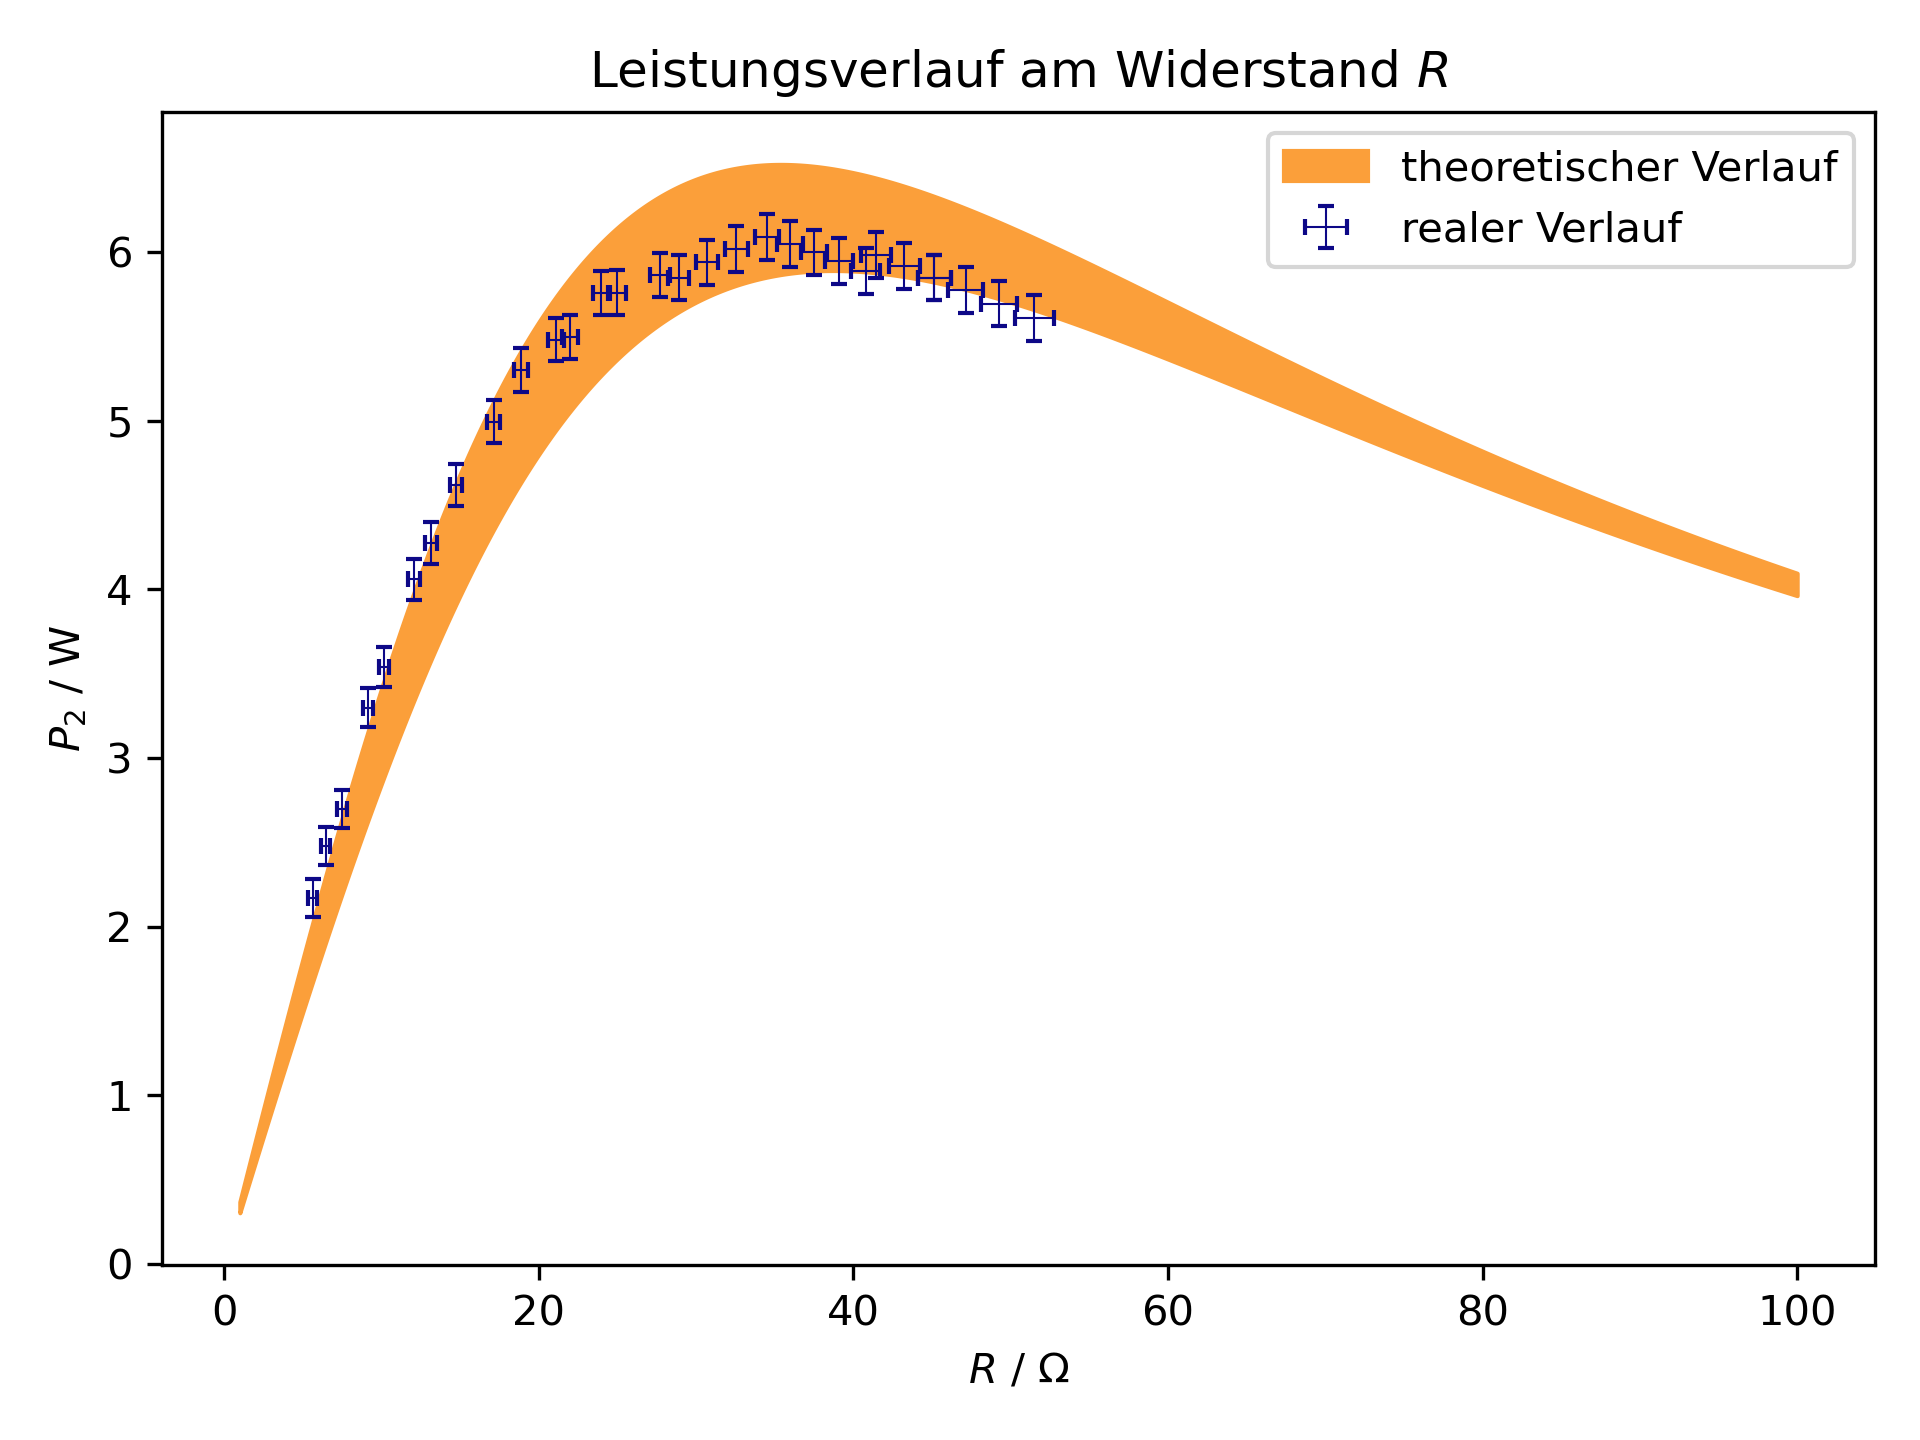
\includegraphics[width=\linewidth]{ausw}
    \caption{Sekundärleistungsverlauf $P_2$ in Abhängigkeit vom Widerstandswert $R$ des Potentiometers $R$. Die realen Werte stammen aus Tab. \ref{tab:auswleistung} und, die theoretischen aus Glg. \ref{eq:auswleistungsverlauf} und Glg. \ref{eq:auswreaktanz}.}
    \label{fig:auswleistung}
\end{figure}



\section{Diskussion}

Die ermittelten Punkte der Wirkleistung $P_2$ und dem Widerstandswert $R$ in Tab. \ref{tab:auswleistung} überlappen mit dem theoretisch zu erwartenden Verlauf, wie in Abb. \ref{fig:auswleistung} zu erkennen ist. Da dies trotz der Vernachlässigung der Kupferwiderstände der Spule $L$ und der Wirkung der Last auf den Transformator der Falls ist, können diese Annahmen gerechtfertigt werden und weiters auf eine fehlerfreie Versuchsdurchführung und Auswertung geschlossen werden. \\

Bei einer erneuten Versuchsdurchführung sollte darauf geachtet werden ein genaueres Wattmeter zu verwenden, da dessen Unsicherheit eine Größenordnung über der Unsicherheit fast aller anderen Messgeräte liegt, und in vier der sechs gesuchten Ergebnisse einfließt.



\section{Zusammenfassung}

Die in Tab. \ref{tab:aufgabe} geforderten Werte wurden berechnet.
\begin{table}[H]
    \centering
    \caption{Die in Tab. \ref{tab:aufgabe} geforderten Werte aus Tab. \ref{tab:auswalles}.}
    \label{tab:zusammenfassung}
    \begin{tabular}{| l | *{3}{SS|}}
        \hline
        Versuch             & \multicolumn{2}{C|}{S_1 \ / \ \si{\va}}   & \multicolumn{2}{C|}{Q_1 \ / \ \si{\var}}  & \multicolumn{2}{C|}{\cos \phi \ / \ 1} \\
        \hline
        Leerlauf            & 17,6  & +-0,5                             & 15,1  & +-1,8                             & 0,51  & +-0,13 \\
        Ohm'sch             & 27,2  & +-1,7                             & 11    & +-9                               & 0,91  & +-0,14 \\
        Ohm'sch-Induktiv    & 25,9  & +-1,7                             & 20    & +-4                               & 0,63  & +-0,12 \\
        \hline
        \hline
        Versuch             & \multicolumn{2}{C|}{P_2 \ / \ \si{\watt}} & \multicolumn{2}{C|}{P_V \ / \ \si{\watt}} & \multicolumn{2}{C|}{\eta \ / \ \si{\percent}} \\
                            \hline
        Leerlauf            &  0    &                                   & 9,0   & +-2,0                             & 0     & \\
        Ohm'sch             & 15,96 & +-0,20                            & 8,8   & +-2,2                             & 0,64  & +-0,06 \\
        Ohm'sch-Induktiv    &  6,09 & +-0,11                            & 10,1  & +-2,2                             & 0,38  & +-0,06 \\
        \hline
    \end{tabular}
\end{table}



\printbibliography
\addcontentsline{toc}{section}{Literatur}



\end{document}
